\documentclass[a4paper,12pt, oneside]{book}

% \usepackage{fullpage}
\usepackage[italian]{babel}
\usepackage[utf8]{inputenc}
\usepackage{amssymb}
\usepackage{amsthm}
\usepackage{graphics}
\usepackage{amsfonts}
\usepackage{listings}
\usepackage{amsmath}
\usepackage{amstext}
\usepackage{colortbl}
\usepackage{engrec}
\usepackage{rotating}
\usepackage{subcaption}
\usepackage{verbatim}
\usepackage[safe,extra]{tipa}
% \usepackage{showkeys}
\usepackage{multirow}
\usepackage{hyperref}
\usepackage{microtype}
% \usepackage{fontspec}
\usepackage{enumerate}
\usepackage{braket}
\usepackage{relsize}
\usepackage{marginnote}
\usepackage{pgfplots}
\usepackage{cancel}
\usepackage{polynom}
\usepackage{booktabs}
\usepackage{enumitem}
\usepackage{framed}
\usepackage{pdfpages}
\usepackage{pgfplots}
\usepackage{algorithm}
\usepackage[backend=biber, backref=true, sorting=none]{biblatex}
\usepackage{fvextra}
\usepackage{csquotes}
% \usepackage{natbib}
% \usepackage{algpseudocode}
% \usepackage[cache=false]{minted}
\usepackage{mathtools}
\usepackage[noend]{algpseudocode}
\usepackage{svg}
\usepackage{graphicx}
\usepackage{hyperref}
\usepackage{setspace}
\usepackage{geometry}
\usepackage{blindtext}
\usepackage{titleps}
\addbibresource{thesis.bib}
\usepackage{tikz}\usetikzlibrary{er}\tikzset{multi  attribute /.style={attribute
    ,double  distance =1.5pt}}\tikzset{derived  attribute /.style={attribute
    ,dashed}}\tikzset{total /.style={double  distance =1.5pt}}\tikzset{every
  entity /.style={draw=orange , fill=orange!20}}\tikzset{every  attribute
  /.style={draw=MediumPurple1, fill=MediumPurple1!20}}\tikzset{every
  relationship /.style={draw=Chartreuse2,
    fill=Chartreuse2!20}}\newcommand{\key}[1]{\underline{#1}}
\usetikzlibrary{arrows.meta}
\usetikzlibrary{decorations.markings}
\usetikzlibrary{arrows,shapes,backgrounds,petri} 
\usetikzlibrary{automata,positioning}
\usetikzlibrary{matrix}
%\renewcommand{\chaptermark}[1]{\markboth{#1}{}}
\usepackage{fancyhdr}
\pagestyle{fancy}

\fancyhead[LO,RE]{\slshape \leftmark}
%\fancyhead[CO,CE]{\slshape\rightmark}
\fancyhead[LE,RO]{\slshape\rightmark}
\fancyfoot[C]{\thepage}
% \fancyhf{}
% \fancyhead[LO,RE]{\slshape \leftmark}
% %\fancyhead[CO,CE]{\slshape\rightmark}
% \fancyhead[LE,RO]{\slshape\thepage}
% \renewcommand{\footrulewidth}{0pt}
%\fancyfoot[C]{\thepage}
% \title{Relazione}
% \fancypagestyle{plain}{% \fancyhf{} % clear all header and footer fields
%   \fancyhead[RO,RE]{\thepage}%RO=right odd, RE=right even
%   \renewcommand{\headrulewidth}{0pt}
%\renewcommand{\footrulewidth}{0.3pt}}


\pgfplotsset{compat=1.13}

\begin{document}

% \maketitle
\newgeometry{margin=1in} 
\begin{titlepage}
  

  \noindent
  \begin{minipage}[t]{0.19\textwidth}
    \vspace{-4mm}{\includegraphics[scale=1.15]{img/logo_unimib.pdf}}
  \end{minipage}
  \begin{minipage}[t]{0.81\textwidth}
    {
      \setstretch{1.42}
      {\textsc{Università degli Studi di Milano - Bicocca}} \\
      \textbf{Scuola di Scienze} \\
      \textbf{Dipartimento di Informatica, Sistemistica e Comunicazione} \\
      \textbf{Corso di laurea in Informatica} \\
      \par
    }
  \end{minipage}
  
  \vspace{40mm}
  
  \begin{center}
    {\LARGE{
        \setstretch{1.2}
        \textbf{Identificazione efficiente di esoni}}}
  \end{center}
  
  \vspace{50mm}

  \noindent
  {\large \textbf{Relatore:} \textit{Prof. Gianluca Della Vedova} } \\

  \noindent
  {\large \textbf{Correlatore:} \textit{Dott. Luca Denti}}
  % \noindent
  % {\large Relatore: \textbf{Prof. Gianluca Della Vedova} } \\

  % \noindent
  % {\large Correlatore: \textbf{Dott. Luca Denti}}
  
  \vspace{15mm}

  \begin{flushright}
    %{\large Relazione della prova finale di:} \\
    % \vspace{1mm}
    % \textbf{\large{Davide Cozzi}} \\
    
    % \large{Matricola 829827}
    \textbf{\large Relazione della prova finale di:} \\
    \large{\textit{Davide Cozzi}}\\
    \large{\textit{Matricola 829827}}
  \end{flushright}
  
  \vspace{40mm}
  \begin{center}
    {\large{\bf Anno Accademico 2019-2020}}
  \end{center}

  \restoregeometry
  
\end{titlepage}
\restoregeometry
\definecolor{shadecolor}{gray}{0.80}
\setlist{leftmargin = 2cm}
\newtheorem{teorema}{Teorema}
\newtheorem{definizione}{Definizione}
\newtheorem{esempio}{Esempio}
\newtheorem{corollario}{Corollario}
\newtheorem{lemma}{Lemma}
\newtheorem{osservazione}{Osservazione}
\newtheorem{nota}{Nota}
\newtheorem{esercizio}{Esercizio}

\algdef{SE}[DOWHILE]{Do}{doWhile}{\algorithmicdo}[1]{\algorithmicwhile\ #1}

\renewcommand{\chaptermark}[1]{%
  \markboth{\chaptername
    \ \thechapter.\ #1}{}}
\renewcommand{\sectionmark}[1]{\markright{\thesection.\ #1}}
\newcommand{\floor}[1]{\lfloor #1 \rfloor}

\newcommand{\MYhref}[3][blue]{\href{#2}{\color{#1}{#3}}}%
\newcommand{\hiddenchapter}[1]{
  \stepcounter{chapter*}
  \chapter*{\arabic{chapter}\hspace{1em}{#1}}
}
% \pagenumbering{roman}

\newpage
\thispagestyle{plain}
\begin{flushleft}
  \huge{\textbf{Abstract}}
\end{flushleft}
\vspace{10mm}
\textit{Con la presente trattazione, ci si propone di descrivere quanto svolto
  durante l'esperienza trimestrale di stage presso l’\textit{Università degli
    Studi di Milano - Bicocca}. Tale esperienza è stata svolta telematicamente
  in collaborazione con il laboratorio di \emph{Bioinformatica e Algoritmica
    Sperimentale}, chiamato
  \emph{\textbf{BIAS}}, del \emph{Dipartimento di Informatica, Sistemistica e
    Comunicazione (\textbf{DISCo})}.\\
  Lo scopo del progetto era la ricerca efficiente di esoni non annotati, detti
  \emph{novel exons}, da integrare nel progetto open source denominato
  \emph{ASGAL}, sviluppato dal gruppo di ricerca del laboratorio stesso, ovvero
  uno strumento 
  atto all'identificazione di eventi di \textit{splicing alternativo}, espressi
  tramite \textbf{RNA-Seq samples}, con l'ausilio dello studio dell'annotazione
  genomica.}
{\pagestyle{plain}
  \tableofcontents
  \cleardoublepage}
\chapter{Introduzione}
\section{Accenni di biologia molecolare}
\subsection{DNA ed RNA}
Prima di iniziare la trattazione più squisitamente computazionale è bene dare
un'introduzione, dal punto di vista biologico, di quanto trattato.\\
Il \textbf{DNA}, sigla corrispondente ad \textbf{acido desossiribonucleico}, è
un acido nucleico contenente le informazioni necessarie al corretto sviluppo di
un essere vivente. Dal punto di vista chimico questa particolare macromolecola
si presenta nella tipica \textbf{struttura a doppia elica}, formata da due
lunghe catene di nucleotidi, dette \textbf{strand}. Nel dettaglio i singoli
nucleotidi sono formati da un \textbf{gruppo fosfato}, dal
\textbf{desossiribosio}, uno \textbf{zucchero pentoso,} e da una \textbf{base
  azotata}. Si hanno, inoltre, 4 tipi diversi di basi azotate:
\begin{enumerate}
  \item \textbf{Adenina}, indicata con la lettera $A$
  \item \textbf{Citosina}, indicata con la lettera $C$
  \item \textbf{Guanina}, indicata con la lettera $G$
  \item \textbf{Timina}, indicata con la lettera $T$
\end{enumerate}
Si hanno quindi due \textbf{strand}, uno detto \textbf{forward
  strand} (indicato solitamente col simbolo ``+'') e uno detto \textbf{backward
  strand} (indicato solitamente col simbolo ``$-$'') che sono direzionati nel verso 
opposto (in termini tecnici si ha che il forward strand va da 5' UTR a 3' UTR,
mentre il backward strand da 3' UTR a 5' UTR) e sono \textit{appaiati} mediante
coppie ben precise di basi azotate.
Infatti, secondo il \textbf{modello di Watson-Crick} (figura \ref{dnaa}), si
ha che:  
\begin{itemize}
  \item l'\textbf{Adenina} si appaia con la \textbf{Timina} e viceversa
  \item la \textbf{Citosina} si appaia con la \textbf{Guanina} e viceversa
\end{itemize}
Questo accoppiamento permette di poter studiare i due \textbf{strand} come uno
``complementare'' all'altro. Infatti, conoscendo la sequenza di basi azotate di
uno \textbf{strand}, è possibile ricavare la sequenza dell'altro mediante la
tecnica del \textbf{Reverse}\&\textbf{Complement} dove, preso uno strand, si
converte ogni sua base secondo il seguente schema:
\begin{itemize}
  \item le $A$ diventano $T$
  \item le $T$ diventano $A$
  \item le $C$ diventano $G$
  \item le $G$ diventano $C$
\end{itemize}
\begin{esempio}
  Vediamo, per completezza, un esempio di
  \textbf{Reverse}\textnormal{\&}\textbf{Complement}.\\ 
  Prendiamo una sequenza genomica $S="\mbox{TAGGCCATATGAC}\,"$ e definiamo la funzione
  $RC(x)$ come la funzione che, presa in ingresso una stringa $x$ costruita
  sull'alfabeto $\Sigma=\{A,C,G,T\}$ (quindi una sequenza genomica), restituisce
  la \textbf{Reverse}\textnormal{\&}\textbf{Complement} della stessa. Si ha
  quindi che: 
  \[RC(S)="\mbox{ATCCGGTATACTG}\,"\]
\end{esempio}
Per riferirci al \textbf{DNA}, contenuto in una data cellula di un essere
vivente, usiamo il termine \textbf{genoma}, che a sua volta viene organizzato in
diversi \textbf{cromosomi}. Si definisce \textbf{gene} una particolare regione
di un \textbf{cromosoma} in grado di codificare una proteina. \\
Ai fini della trattazione del progetto, è necessario introdurre anche
l'\textbf{RNA}, sigla corrispondente ad \textbf{acido ribonucleico} (avendo il
\textbf{ribosio} come zucchero pentoso), ovvero una
molecola, simile al \textbf{DNA}, dotata di una singola 
catena nucleotidica, sempre con 4 tipi di basi azotate (anche se si ha
l'\textbf{Uracile}, che si indica con la lettera $U$, al posto della
\textbf{Timina}). Tra i compiti dell'\textbf{RNA} si ha quello della codifica e
decodifica dei \textbf{geni}.
\begin{figure}[H]
  \centering
  \includesvg[scale = 0.8]{img/dna.svg}
  \caption{Rappresentazione grafica del DNA \cite{dna}.}
  \label{dnaa}
\end{figure}
\subsection{Esoni, Introni e Splicing alternativo}
Per ottenere una \textbf{proteina} da un \textbf{gene} si hanno 3 passaggi
(rappresentati nella figura \ref{prot}):
\begin{enumerate}
  \item La \textbf{trascrizione}, fase dove la sequenza del gene è copiata
  nel \textbf{pre-messenger RNA (pre-mRNA)}. Nel dettaglio viene selezionato uno
  dei due strand del gene e un enzima, chiamato \textbf{RNA Polimerasi}, procede
  alla trascrizione della sequenza selezionata creando il \textbf{pre-mRNA}. In
  questa fase la \textit{Timina} viene sostituita dall'Uracile. È bene
  introdurre subito che in questo progetto non si terrà mai conto, a fini di
  semplificazione, del passaggio tra Timina e Uracile in quanto verrà usata
  sempre la \textit{Timina}.
  \item Lo \textbf{splicing}, fase dove vengono rimosse le parti non codificanti
  dalla molecola di \textbf{pre-mRNA}, formando il \textbf{messenger RNA
    (mRNA)},
  detto anche \textbf{trascritto}. Per poter trattare al meglio questa fase
  bisogna parlare in primis di \textbf{esoni} e \textbf{introni}. In prima
  analisi si potrebbe dire, peccando di precisione, che gli
  \textbf{esoni} sono le sezioni codificanti di un gene mentre gli
  \textbf{introni} sono le porzioni non codificanti. Solo gli esoni formano il
  trascritto. Si ha, inoltre, che le prime due basi di un introne sono dette
  $5'$, nell'uomo solitamente si ha la coppia $GT$, mentre le ultime due,
  solitamente $AG$ nell'uomo, sono
  dette $3'$ e sono meglio identificate come \textbf{siti di taglio (splice
    sites)}. 
  Quindi un esone, in realtà, non coincide esattamente con una regione
  codificante, detta \textbf{CDS}, a causa di queste particolari coppie di
  basi. Si notifica però che, come spesso accade, i termini vengono usati in
  sovrapposizione. 
  \newpage
  \item La \textbf{traduzione}, fase dove viene effettivamente codificata la
  proteina a partire da una sezione dell'\textbf{m-RNA}. 
  Bisogna quindi nominare particolari sequenze nucleotidiche di cardinalità 3: i
  \textbf{codoni}. Tali triplette sono tradotte in amminoacidi che, concatenati,
  formano le proteine. Esistono particolari codoni che sono utili al fine
  di riconoscere l'inizio e la fine della \textit{sintesi proteica}. In
  particolare si ha un codone d'inizio, detto \textbf{start codon}, che
  solitamente corrisponde alla tripletta \textit{AUG}, mentre, per il codone di
  fine, detto \textbf{stop codon}, solitamente si ha una tripletta tra
  \textit{UAA}, \textit{UAG} e  \textit{UGA}.
\end{enumerate}
Ai fini di questo progetto ci si concentra sullo \textbf{splicing}.\\
\begin{figure}
  \centering
  \includesvg[scale = 0.58]{img/tst.svg}
  \caption{Rappresentazione grafica delle tre fasi per la sintesi di una
    proteina. Abbiamo all'inizio un ingrandimento al fine di poter visualizzare
    la \textit{trascrizione} con la produzione di 
    \textit{pre-mRNA} a partire dal \textit{DNA}. Seguono poi, allontanando nel
    disegno il ``campo visivo'', un evento di splicing ``regolare''
    (dove semplicemente vengono rimossi gli introni, in verde) e l'ottenimento
    del trascritto. Infine, riavvicinando nuovamente la ``visuale'', si ha un
    ipotetico pezzo di proteina, ottenuto con la \textit{traduzione} di tale
    trascritto, dove vengono segnalati anche i codoni.}    
  \label{prot}
\end{figure}

In realtà, un gene è in grado di sintetizzare più di una proteina
mediante il cosiddetto \textbf{splicing alternativo}, che consiste in diverse
varianti dell'evento di splicing al fine di ottenere diversi trascritti. Si
descrivono le principali modalità di splicing alternativo, visualizzabili
nella figura \ref{alt}:
\begin{itemize}
  \item L'\textbf{exon skipping}, ovvero \textit{salto dell'esone}, dove un
  esone 
  (o anche più esoni) può essere escluso dal trascritto primario oppure dove un
  nuovo esone (o più nuovi esoni) può essere incluso nello stesso. 
  \item L'\textbf{alternative acceptor site}, ovvero \textit{sito di taglio
    alternativo $3'$}, dove una parte del secondo esone può essere considerata
  non codificante o, alternativamente, una porzione dell'introne adiacente può
  essere considerata codificante.
  \item L'\textbf{alternative donor site}, ovvero \textit{sito di taglio
    alternativo $5'$}, dove una parte del primo esone viene considerata non
  codificante o, alternativamente, una porzione di introne adiacente può
  essere considerata codificante.
  \item I \textbf{mutually exclusive exons}, ovvero \textit{esoni mutuamente
    esclusivi}, dove solo uno di due esoni viene conservato nel trascritto.
  \item L'\textbf{intron retention}, ovvero \textit{introne trattenuto}, dove un
  certo introne viene incluso nel trascritto primario.
\end{itemize}
Le varie modalità di splicing alternativo non si escludono a vicenda, rendendo
lo studio di tale fenomeno assai complesso.\\
Il progetto \textbf{ASGAL} \cite{denti} \cite{asgal}
(\textit{\textbf{A}lternative \textbf{S}plicing \textbf{G}raph
  \textbf{AL}igner}) è nato con lo scopo di studiare, dal punto di vista
computazionale, tali eventi e il progetto descritto in questa trattazione si
occupa di studiare eventi che considerino porzioni teoricamente non
codificanti come codificanti. 
\begin{figure}
  \centering
  \includegraphics[scale = 0.5]{img/sedenti.jpg}
  \caption{Schema riassuntivo per gli eventi di splicing alternativo
    \cite{denti}.}
  \label{alt}
\end{figure}

\chapter{Preliminari}
Passiamo ora alla spiegazione di alcuni concetti e di alcune nozioni necessarie
a comprendere al meglio la natura del progetto.
\section{Formato dei files}
Nel campo della bioinformatica vengono usati particolari formati di files di
testo per la memorizzazione delle più svariate nozioni necessarie in questo
ambito. In questa sezione si andranno quindi ad analizzare, in base agli scopi,
i formati usati durante il progetto.
\subsection{Genoma e RNA-Seq sample}
Come abbiamo visto una sequenze nucleotidica può essere facilmente rappresentata
mediante una stringa creata a partire dall'alfabeto $\Sigma=\{A,C,G,T\}$, dove ogni
lettera corrisponde all'iniziale di una delle 4 basi azotate del DNA.\\
Per poter memorizzare una sequenza nucleotidica viene usato un file
\textbf{FASTA} \cite{fasta} (solitamente indicato con l'estensione
\texttt{.fa}), il cui contenuto è piuttosto minimale in quanto conta
essenzialmente di due sole parti:
\begin{enumerate}
  \item un \textit{header}, specificato all'inizio dal carattere ``>'',
  contenente un'indicatore univoco per identificare la sequenza nucleotidica ed
  eventualmente informazioni aggiuntive
  \item una \textit{stringa} rappresentante la sequenza nucleotidica
\end{enumerate}
In questo progetto il genoma di riferimento, per esempio quello relativo ad un
certo cromosoma, è contenuto in un file FASTA.\\
In un file FASTA è anche possibile memorizzare più di una sequenza nucleotidica,
concatenando headers e stringhe. In questo progetto le reads da allineare (il
nostro \textbf{RNA-Seq sample}) sono anch'esse contenute in un file FASTA.
\begin{esempio}
  Vediamo un esempio relativo ad una porzione di un file FASTA con due sequenze
  nucleotidiche: 
\begin{verbatim}
>FBtr0070103_e_5224_X_289258
TGTTTCTACCAACCTTATCACGCTTTGGCTTATCCTCGGCATTGTCGTCCTTCATAAACG
AGGGCTGCAGGCTGAATCGGCGGCGTAAGTGGCGGCCACG
>FBtr0070103_e_2113_X_289177
ACGTTTTTCCCACTTTTGCAGAGCCCATGACGACGATTTTGTGGCGTGCGTTGGCCGGTC
CAATGGCATCATCTACCGCGTTGTTTCTACCAACCTTATC
\end{verbatim}
\end{esempio}
\subsection{Annotazione}
Come abbiamo discusso nell'introduzione, la struttura di un gene è alquanto
complessa e viene rappresentata mediante un insieme di \textbf{features}, detto
\textit{annotazione}. Questo 
insieme di features viene spesso memorizzato all'interno di un file
\textbf{GTF} \cite{gtf} (solitamente indicato con l'estensione
\texttt{.gtf}). Ogni singola feature viene rappresentata da 9 campi, delimitati
da \textbf{tabulazioni} (``$\backslash$t''): 
\begin{enumerate}
  \item l'identificativo del cromosoma in cui è stata localizzata la feature
  \item l'identificativo della sorgente da cui proviene l'annotazione,
  tipicamente il nome della banca dati o del software utilizzato 
  \item il tipo di feature, per esempio \textit{gene, transcript, exon, start
    codon, stop codon, CDS}$\ldots$
  \item la coordinata di partenza della feature nel genoma di riferimento
  \item la coordinata di fine della feature nel genoma di riferimento
  \item il grado di confidenza relativo all'esistenza della feature e alle sue
  coordinate. Qualora il dato non fosse disponibile si avrà un ``.'' al suo
  posto 
  \item lo strand della feature, indicato con ``+'' o ``$-$''
  \item il frame della feature, indicante quale base della feature stessa è la
  prima base del codone. Qualora il dato non fosse disponibile si avrà un ``.''
  al suo posto
  \item una lista, opzionale, di informazioni aggiuntive, tra loro separate dal
  carattere ``;''
\end{enumerate}
\begin{esempio}
  Vediamo un esempio di feature, relativa a un esone, estratta da un file GTF
  (per comodità sono state omesse le informazioni aggiuntive):
\begin{verbatim}
X FlyBase exon 287329 287526 . - . informazioni divise da ";"	

\end{verbatim}
\end{esempio}
\subsection{Allineamenti}
Le sequenze nucleotidiche (nel nostro caso le sequenze contenute nelle reads)
allineate a un genoma di riferimento vengono memorizzate in un file \textbf{SAM
  (\textit{Sequence Alignment Map})} \cite{sam} (solitamente indicato con
l'estensione \texttt{.sam}). La struttura di questo formato è complessa e conta
di un header, contenente alcune informazioni relative al formato del file stesso
e alle sequenze, e di una sezione dedicata all'allineamento, che viene a sua
volta divisa in 11 parti, tra cui l'identificatore della read e del genoma di
riferimento, le coordinate di inizio allineamento, la stringa CIGAR e la
sequenza della read. Di queste parti quella che più ci interessa è la stringa
\textbf{CIGAR (\textit{Concise Idiosyncratic Gapped Alignment Report})} che
consiste in una rappresentazione compressa dell'allineamento. In una CIGAR si
hanno coppie concatenate di numeri interi e operatori, dove l'operatore, nel
dettaglio un carattere, rappresenta un determinato evento mentre l'intero che lo
precede rappresenta il numero di occorrenze di tale evento. Tra gli operatori
principali ricordiamo: 
\begin{itemize}
  \item ``M'' per i match
  \item ``D'' per le rimozioni
  \item ``I'' per gli inserimenti
  \item ``S'' per quelle parti che non compaiono nell'allineamento
\end{itemize}
\begin{esempio}
  Vediamo l'esempio di una riga di un file SAM rappresentante un match perfetto,
  essendo la read lunga 100:
\begin{verbatim}
FBtr0342963_e_896_X_289053 16 X 289054 255 100M * 0 0	
GCAGTGTCCAAAATATCAAGGGTAAGGCTCACGCTGGCGATGGAAAAGTTGCCTTGGTGCA
TTTCCTCAATGGTCCGCTTGTACTTGGTGCTAAATGTAT	*	NM:i:1
\end{verbatim}
\end{esempio}
Una rappresentazione binaria delle informazioni di un file \textbf{SAM} può
essere contenuta in un file \textbf{BAM (\textit{Binary Alignment Map})}
\cite{sam} 
\section{Splicing graph}
La prima struttura dati che andiamo a descrivere è lo \textbf{splicing
  graph} \cite{denti}.\\ 
Innanzitutto, riprendendo i concetti di biologia molecolare
descritti all'inizio, bisogna formalizzare in termini più matematici e
computazionali il concetto di \textbf{trascritto}. Possiamo quindi dire che un
trascritto $T$ è una sequenza di coppie $[b_i,e_i]$ dove ciascuna coppia
rappresenta un determinato esone, mediante le coordinate di inizio e fine nel
genoma di riferimento. Si ha quindi che:
\[T=\langle[b_1,e_1],[b_2,e_2],\ldots, [b_n,e_n]\rangle\]
Sfruttando la definizione computazionale di esone possiamo definire anche
quella di introne. Sapendo infatti che l'i-esimo esone è rappresentato tramite
$[b_i,e_i]$, possiamo definire anche l'introne compreso tra l'i-esimo esone e il
suo successore come:
\[[e_i+1,b_{i+1}-1]\]
Possiamo, quindi, definire lo \textbf{splicing graph} di un gene come il
\textbf{grafo diretto aciclico \textit{(DAG)}} $S_G=(\varepsilon_G, E)$, con
$\varepsilon_G$ insieme degli esoni e $E$ insieme degli archi che connettono i
nodi relativi a due
esoni consecutivi in almeno un trascritto. In aggiunta vengono collegati,
mediante archi diversi da quelli di $E$, i nodi relativi a due esoni che non
sono consecutivi in alcun trascritto tali per cui il primo sia completamente a
sinistra rispetto al secondo nel genoma di riferimento. Questi particolari archi
sono chiamati \textbf{novel edges} (figura \ref{sg}). In termini computazionali,
nella 
\textit{matrice di adiacenza} del grafo, si avrà il valore 
$2$ per tali archi. \\  
\begin{figure}[H]
  \centering
  \includesvg[scale = 0.6]{img/sgnt.svg}
  \caption{Esempio di splicing graph su 4 esoni (in cui si ipotizza un trascritto
    dove è assente l'esone 3), con gli archi in blu e i novel edges in
    verde tratteggiato.} 
  \label{sg}
\end{figure}
\subsection{Linearizzazione dello splicing graph}
Spostiamo quindi l'attenzione sulle sequenze nucleotidiche, individuabili nel
genoma di riferimento tramite le coordinate degli esoni che etichettano ogni
nodo dello \textbf{splicing graph}.\\
Definiamo la \textbf{linearizzazione dello splicing graph} come la
concatenazione delle etichette dei singoli nodi, precedute da un carattere
sentinella, che, in primis per motivazioni computazionali di rappresentabilità
nel codice, viene identificato mediante il carattere ``|''. Tale carattere viene
aggiunto anche alla fine della linearizzazione, che, per comodità, chiamiamo
$Z$. 
\begin{esempio}
  Ipotizziamo di avere 3 esoni consecutivi etichettati $\mbox{TAT}$,
  $\mbox{GCGCT}$ e $\mbox{TGA}$. Si ha che la loro linearizzazione, usando il
  carattere ``$|$'' come carattere sentinella, è:
  \[|\mbox{TAT}\,|\mbox{GCGCT}\,|\mbox{TGA}\,|\]
\end{esempio}
Per poter comprendere l'utilità della linearizzazione dobbiamo prima introdurre
un ulteriore concetto, quello di \textit{bit vector}.
\section{Bit vector}
Un \textbf{bit vector} è un array, di lunghezza definita, formato da elementi
binari. Chiamiamo $B$ il bit vector di lunghezza $n$. Si ha che:
\[B[i]\in\{0,1\},\,\forall\, i=0,\ldots,n-1\]
Questa particolare struttura dati permette due operazioni estremamente utili, la
\textbf{rank} e la \textbf{select}. Un'implementazione \textit{naive} di queste
funzioni richiederebbe un tempo $O(n)$ ma, con l'ausilio di $o(n)$ bits
aggiuntivi in memoria, si riesce a raggiungere una complessità temporale
costante $O(1)$.
% cit ad alex bowe
\subsection{Rank}
La prima operazione è la \textbf{rank} che permette di calcolare, in un
\textit{bit vector} di $n$ elementi, il numero di occorrenze di 1 tra la
posizione 0 e una posizione $x$ passata come argomento alla funzione,
quest'ultima esclusa. Formalmente si ha:
\[\mathtt{rank}(x)=\sum_{i=0}^{x-1}B[i],\,\,0\leq x< n\]
\subsection{Select}
La seconda operazione è la \textbf{select} che permette di calcolare, in un
\textit{bit vector} di $n$ elementi, l'indice dell'$x$-esimo 1. Formalmente si
ha: 
\[\mathtt{select}(x)=\max\{j<n\,|\,\,\,\mathtt{rank}(j)\leq x\},\,\,0<x\leq
  \mathtt{rank}(n)\] 

\begin{esempio}
  Ipotizziamo di avere il seguente bit vector $B$:
  \begin{center}
    \begin{tikzpicture} [nodes in empty cells,
      nodes={minimum width=0.6cm, minimum height=0.6cm},
      row sep=-\pgflinewidth, column sep=-\pgflinewidth]
      border/.style={draw}
      
      \matrix(vector)[matrix of nodes,
      row 1/.style={nodes={draw=none, minimum width=0.3cm}},
      nodes={draw}]
      {
        \tiny{0} & \tiny{1} & \tiny{2} & \tiny{3} & \tiny{4} & \tiny{5} & \tiny{6}
        & \tiny{7} & \tiny{8} & \tiny{9} & \tiny{10} & \tiny{11} & \tiny{12} &
        \tiny{13}\\  
        $\mathbf{1}$ & $0$ & $0$ & $\mathbf{1}$ & $0$ & $\mathbf{1}$ & $0$ &
        $\mathbf{1}$ & $0$ & $\mathbf{1}$ & $0$ & $0$ & $\mathbf{1}$ & $0$\\ 
      };
    \end{tikzpicture}
  \end{center}
  Si ha che, per esempio:
  \[\mathtt{rank}(6)=3\]
  \[\mathtt{select}(5) =9\]
\end{esempio}
\subsection{Corrispondenza tra linearizzazione e bit vector}
Tornando quindi alla linearizzazione $Z$ (con carattere sentinella ``|'') dello
\textbf{splicing graph}, notiamo che è possibile associare alla stessa un
\textit{bit vector} $B$, di pari lunghezza $n$, tale che:
\[
  \begin{cases}
    B[i] = 1 &\mbox{ sse } Z[i] = \,"|"\,\\
    B[i] = 0 &\mbox{ altrimenti}
  \end{cases}
\]
In questo modo, mediante l'operazione \texttt{rank}, si può calcolare
l'\textit{ID} dell'esone corrispondente ad un certo indice della linearizzazione
mentre, grazie alla \texttt{select}, è possibile calcolare l'indice di partenza
sulla linearizzazione di un determinato esone (passando alla \texttt{select} il
suo \textit{ID}). Si può, inoltre, fare una considerazione aggiuntiva sulla
\texttt{select}: considerando la \texttt{select} di un esone e dell'esone che
risulta essere rappresentato mediante il successore dell'\textit{ID} del primo,
è possibile calcolare l'indice di partenza e l'indice di fine dell'esone stesso
nella linearizzazione, in modo da poterne estrarre la sequenza. Nel dettaglio
bisogna considerare anche il carattere ``sentinella'' 
quindi, in realtà, per l'i-esimo esone si ha che il suo indice di partenza sulla
linearizzazione è $\mathtt{select}(i)+1$ e quello di fine è
$\mathtt{select}(i+1)-1$. L'utilità della \texttt{rank} verrà trattata più
avanti nel testo.   
\begin{esempio}
  Vediamo quindi un esempio di come viene mappato un bit vector per la
  linearizzazione:
  \[|AT|G|T|C|GC|A|\]
  \begin{center}
    \begin{tikzpicture} [nodes in empty cells,
      nodes={minimum width=0.6cm, minimum height=0.6cm},
      row sep=-\pgflinewidth, column sep=-\pgflinewidth]
      border/.style={draw}
      
      \matrix(vector)[matrix of nodes,
      row 1/.style={nodes={draw=none, minimum width=0.3cm}},
      row 3/.style={nodes={draw=none, minimum width=0.3cm}},
      nodes={draw}]
      {
        \tiny{0} & \tiny{1} & \tiny{2} & \tiny{3} & \tiny{4} & \tiny{5} &
        \tiny{6} & \tiny{7} & \tiny{8} & \tiny{9} & \tiny{10} & \tiny{11} &
        \tiny{12} & \tiny{13} & \tiny{14}\\
        $\mathbf{1}$ & $0$ & $0$ & $\mathbf{1}$ & $0$ & $\mathbf{1}$ & $0$ &
        $\mathbf{1}$ & $0$ & $\mathbf{1}$ & $0$ & $0$ & $\mathbf{1}$ & $0$ &
        $1$\\
        {|} & {A} & {T} & {|} & {G} & {|} & {T} & {|} & {C} & {|} & {G} & {C} &
        {|} & {A} & {|}\\   
      };
    \end{tikzpicture}
  \end{center}
  Possiamo quindi dire che, ipotizzando di aver calcolato la linearizzazione
  dello \textbf{splicing graph}, per esempio, la base $T$, all'indice 6,
  appartiene al terzo esone. Inoltre, si ha che il quinto esone parte all'indice
  9 (non contando il carattere sentinella dall'indice 10). Infatti, usando le
  due operazioni sopra descritte, si ha che:
  \[\mathtt{rank}(6)=3\]
  \[\mathtt{select}(5) =9\]
\end{esempio}

\section{Allineamento}
Il passo successivo, nella pipeline di ASGAL, consiste
nell'\textbf{allineamento} di ciascuna read dell'\textbf{RNA-Seq sample} con lo
\textbf{splicing graph}. A tal fine bisogna però introdurre il concetto di
\textbf{MEM}. 
\subsection{Maximal Exact Matches}
\begin{definizione}
  Un \textbf{Maximal Exact Match (\textit{MEM})} \cite{mem} è definito come la
  più lunga sottostringa comune a due stringhe tale che non possa essere estesa
  in alcuna direzione senza aggiungere un mismatch. \\
  Date due stringhe $T$ e $P$, rispettivamente di lunghezza $N$ e $M$, un
  \textbf{MEM} tra queste due stringhe è definito dalla tripla:
  \[m=(t,p,l)\]
  dove:
  \begin{itemize}
    \item \textit{\textbf{t}} è l'indice di partenza del \textbf{MEM} sulla
    stringa $T$, quindi si ha che $0\leq t< N$
    \item \textit{\textbf{p}} è l'indice di partenza del \textbf{MEM} sulla
    stringa $P$, quindi si ha che $0\leq p< M$ 
    \item \textit{\textbf{l}} è la lunghezza del \textbf{MEM}
  \end{itemize}
\end{definizione}
\begin{esempio}
  Vediamo un esempio chiarificatore \cite{denti}.\\
  Siano $T=MISSISSIPPI$ e $P=MIPPISSI$, calcolando i \textbf{MEMs} di lunghezza
  $l\geq 2$, si ottiene un insieme di \textbf{MEMs} contenente:
  \begin{itemize}
    \item $(0,0,2)$, rappresentante la stringa $MI$
    \item $(1,4,4)\,\,e\,\,(4,4,4)$, rappresentanti la stringa $ISSI$
    \item $(7,1,4)$, rappresentante la stringa $IPPI$
  \end{itemize}
\end{esempio}
\noindent
Si può quindi facilmente notare come il calcolo dei \textbf{MEMs} sia 
fondamentale nello studio di allineamenti tra un genoma (o una sua sottoparte
come nel nostro caso) e un insieme di reads.\\
Qualora si abbia un \textbf{MEM} ``parziale'' non estendibile solo a destra si
parla di \textbf{Right MEM}.\\
Senza entrare nel dettaglio, possiamo dire che ASGAL basa il calcolo dei
\textbf{MEMs} su un algoritmo \cite{mem} che riesce a calcolare l'insieme di
\textbf{MEMs} (di lunghezza minima arbitraria pari a $L$), tra due stringhe $T$
e $P$, rispettivamente di lunghezza $N$ e $M$, in:  
\[O(M+z+k\cdot w)\]
dove:
\begin{itemize}
  \item $z$ è il numero di right \textbf{MEMs} di lunghezza $\geq L$
  \item $k$ è il numero di \textbf{MEMs} di lunghezza $\geq L$
  \item $w$ rappresenta il tempo di accesso all'\textit{indice} della stringa
  $T$ (in quanto l'algoritmo si basa sull'\textit{indicizzazione} di tale
  stringa) 
\end{itemize}
Procedendo con il calcolo dei \textbf{MEMs}, tra ogni singola read $R$ e la
\textbf{linearizzazione dello splicing graph} $Z$, si nota subito che ogni
\textbf{MEM} può cadere all'interno di un solo nodo del grafo, ovvero
all'interno di un solo esone, grazie al carattere ``sentinella'' presente solo
nella linearizzazione.\\ 
Sfruttiamo ora quanto discusso in merito alla linearizzazione per studiare
meglio l'allineamento. Si ha che il \textbf{MEM} $m=(i_Z, i_R, l)$ appartiene
all'i-esimo nodo dello splicing graph, calcolabile tramite
$\mathtt{rank}(i_Z)$. Ai fini della trattazione è necessario anche stabilire una
relazione d'ordine tra due \textbf{MEMs}. Ipotizzando quindi di aver calcolato
anche $m'=(i_Z',i_R',l')$ viene stabilita una relazione d'ordine tra $m$ e $m'$
tale per cui $m$ precede $m'$ sulla read $R$ sse:
\[i_R<i_R'\,\,\,\land\,\,\, i_R+l<i_R'+l'\]
e tale precedenza viene indicata con la notazione:
\[m\prec_R m'\]
Lo stesso ragionamento viene fatto su $Z$, ottenendo la relazione $\prec_Z$, ma
solo se i due \textbf{MEMs} appartengono allo stesso nodo dello splicing graph,
ovvero se $\mathtt{rank}(i_Z)==\mathtt{rank}(i_Z')$. 

\subsection{MEMs graph}
In ASGAL, si basa lo studio dei \textbf{MEMs}, calcolati tra la linearizzazione
dello \textbf{splicing graph} $Z$ e la read $R$, sullo studio di un grafo,
orientato e pesato, detto \textbf{MEMs graph}. Chiamato $M$ l'insieme dei
\textbf{MEMs} calcolati si ha che il grafo è così definito: 
\[G_M=(M,E_M)\]
dove, quindi, i vertici sono i \textbf{MEMs} stessi. Due nodi sono collegati da
un arco sse, in primis, il nodo di partenza è etichettato da un \textbf{MEM}
precedente, secondo la relazione $\prec_R$, a quello di arrivo. Oltre a questa
condizione necessaria serve un'altra tra sei condizioni che possono essere
visualizzate nella figura \ref{fig:mem}.\\
All'inizio della computazione si ha, inoltre, la presenza di due nodi, uno detto
\textbf{nodo start} e uno detto \textbf{nodo end}, etichettati, rispettivamente,
con il \textbf{MEM} $m=(0,0,0)$ e con il \textbf{MEM} $m=(-1,-1,-1)$. Tali nodi
vengono usati come base per la costruzione del grafo stesso. I criteri verranno
approfonditi più avanti nella trattazione.\\ 
Al fine di calcolare il vero e proprio allineamento della read viene quindi
visitato il \textbf{MEMs graph} cercando, qualora siano calcolabili, i
\textbf{cammini   minimi} (con peso massimo arbitrario), mediante il famoso
\textbf{algoritmo di Dijkstra}, tra il \textit{nodo start} e il \textit{nodo
  end}, ottenendo una o più liste di \textbf{MEMs} rappresentanti
l'allineamento.   
\begin{figure}
  \centering
  \includegraphics[scale = 0.45]{img/mg.png}
  \caption{Rappresentazione grafica \cite{denti} delle possibili situazioni
    riscontrabili 
    nello studio dei \textbf{MEMs}. Un arco tra il \textbf{MEM} $m$ e
    il \textbf{MEM} $m'$ viene aggiunto solo in presenza di determinate
    circostanze, a seconda che i due \textbf{MEMs} si trovino o meno sullo
    stesso esone, se abbiano o meno delle sovrapposizioni o se siano troppo
    distanti tra loro (analizzando i \emph{gaps} sulla read e
    sulla linearizzazione, detti, rispettivamente, $sgap_R$ e $sgap_z$, nonché
    eventuali suffissi e prefissi delle sequenze esoniche). Tali circostanze
    sono analizzate, in modo approfondito, nello studio del dottor Luca Denti
    \cite{denti}.}  
  \label{fig:mem}
\end{figure}
\section{Pipeline di ASGAL}
Per concludere il capitolo è bene schematizzare la pipeline completa di ASGAL.
\begin{figure}
  \centering
  \includegraphics[scale = 0.5]{img/pipe.jpg}
  \caption{Rappresentazione schematica della pipeline di ASGAL \cite{denti}}
  \label{fig:pip}
\end{figure}
Analizzando lo schema, rappresentato in figura \ref{fig:pip}, si ha,
innanzitutto, la costruzione dello \textbf{splicing graph} a partire dal genoma
di riferimento e dall'annotazione relativa a un singolo gene dello
stesso. Durante questa fase viene prodotto anche un particolare file, di un
formato custom, detto \texttt{.gtf.sg}, contenente informazioni sullo
\textbf{splicing graph}. Avremo quindi all'interno di tale file: 
\begin{itemize}
  \item indicazioni sulla provenienza del genoma, sulla sua lunghezza ed
  eventualmente sullo strand
  \item la stringa relativa alla linearizzazione calcolata tramite lo
  \textbf{splicing graph}
  \item la matrice di adiacenza relativa allo \textbf{splicing graph} (dove con
  1 vengono indicati gli archi \textit{normali} mentre con 2 vengono indicati i
  \textit{novel edges})
  \item la lista contenente le posizioni di inizio e fine degli esoni, ordinati
  secondo l'ordine di aggiunta allo \textbf{splicing graph}. Si ha, quindi,
  il medesimo ordine degli \textit{ID} utilizzabili con le operazioni di
  \texttt{rank} e \texttt{select} in quanto tale ordine corrisponde anche
  all'ordine con cui sono state concatenate le corrispondenti sequenze, per
  ottenere la \textbf{linearizzazione dello splicing graph}
\end{itemize}
Si procede quindi con l'allineamento dello \textbf{splicing graph}
con le varie read presenti nell'\textbf{RNA-Seq sample}, tramite lo studio del
\textbf{MEMs graph}, studiando, per ogni read, anche il suo
\textbf{Reverse}\&\textbf{Complement}. Anche in questo caso, il risultato di
tale procedura viene salvato in un particolare file di formato custom con
estensione \texttt{.mem} che conterrà, per ogni riga:
\begin{itemize}
  \item lo strand su cui è stato calcolato l'allineamento
  \item il nome della read allineata
  \item il punteggio relativo alla qualità dell'allineamento, corrispondente al
  peso del cammino della lista di \textbf{MEMs} nel \textbf{MEMs graph} 
  \item la lista dei \textbf{MEMs} rappresentanti l'allineamento con lo
  \textbf{splicing graph}
  \item l'intera sequenza della read
\end{itemize}
A questo punto, tramite diversi scripts, si procede alla costruzione del file
\textbf{SAM} e al calcolo degli eventi di \textbf{splicing alternativo} (salvati
in un file di formato \textbf{CSV} (\textit{Comma-Separated Values})).
\chapter{Metodo}
Si discute ora della vera e propria ricerca dei cosiddetti \textit{novel exons},
ovvero potenziali esoni non presenti nell'annotazione, che vengono però allineati
da determinate read dell'\textbf{RNA-Seq sample}. A tal fine, sono state
effettuate diverse aggiunte alla \textit{codebase} preesistente di ASGAL e
quindi è bene, come prima cosa, analizzare le strumentazioni, ovvero i linguaggi
di programmazione e le librerie principali, usate nel progetto.
\section{Introduzione agli strumenti usati}
\subsection{Linguaggi e librerie}
Navigando il codice sorgente di ASGAL, si nota subito come ci sia una divisione
netta tra due sezioni:
\begin{enumerate}
  \item Una prima sezione contenente codice scritto in \textit{C++}, atto a
  calcolare il vero e proprio allineamento e alla produzione del file
  \texttt{.mem}, contenuto nella cartella \texttt{/src}.
  \item Una seconda sezione contenente diversi scripts in \textit{Python} atti a
  gestire l'intera pipeline e a studiarne i risultati (studiando in primis il
  file \texttt{.mem}). Gli scripts in \textit{Python} sono contenuti nella
  cartella \texttt{/script}.
\end{enumerate}
Ai fini del calcolo dei \textit{novel exons} non sono stati aggiunti nuovi
sorgenti per la parte in \textit{C++}, in quanto sono state effettuate solo
aggiunte e modifiche all'interno della \textit{codebase}. Si ha infine uno
script in \textit{Python}, denominato \texttt{asgal}, che gestisce
l'intero processo di calcolo, concatenando i codici in \textit{C++} e i vari
scripts in \textit{Python}.\\ 
Bisogna, quindi, citare una serie di librerie esterne utilizzate in diverse
parti del codice \textit{C++}:
\begin{itemize}
  \item La libreria \textbf{LEMON (\textit{Library for Efficient
      Modeling and Optimization in Network})} \cite{lemon}, che fornisce tutte
  le strumentazioni necessarie a lavorare con i grafi, a partire da classi per
  gestire grafi orientati e pesati fino a metodi per studiarne il cammino
  minimo, mediante algoritmi, come quello di \textbf{Dijkstra} citato
  precedentemente. Questa libreria, scritta in \textit{C++}, viene usata per
  gestire il \textbf{MEMs graph}, per la sua creazione, per la sua estensione e
  per il calcolo dei cammini minimi.
  \item La libreria \textbf{Klib} \cite{klib}, che fornisce, in una delle sue
  svariate componenti indipendenti tra loro, metodi efficienti per
  il \textit{parsing} e per l'accesso a files in formato \textit{FASTA}.
  La componente principale usata nella \textit{codebase} è
  \texttt{kseq.h}. Questa libreria, scritta in  \textit{C}, viene utilizzata
  per gestire i due files contenenti il genoma di riferimento e l'\textbf{RNA-Seq
    sample}.
  \item La libreria \textbf{Sdsl-lite} \cite{sdsl}, che fornisce
  l'implementazione di diverse \textbf{strutture dati succinte}, tra cui una
  struttura dati per il \textit{bit vector}, comprensiva delle due operazioni
  \texttt{rank} e \texttt{select}, implementate nella libreria per essere
  estremamente efficienti. 
\end{itemize}
Per quanto riguarda il codice \textit{Python} abbiamo invece un uso frequente
di due librerie esterne:
\begin{itemize}
  \item \textbf{Biopython} \cite{biopython} per la lettura e il
  \textit{parsing} dei files \textit{FASTA}
  \item \textbf{Gffutils} \cite{gffutils} per la lettura, il
  \textit{parsing} e la manipolazione delle annotazioni contenute nei files
  \textit{GTF} 
\end{itemize}
\subsection{Snakemake}
Un altro strumento utilizzato in questo progetto, durante la fase di
sperimentazione, è stato
\textbf{Snakemake} \cite{10.1093/bioinformatics/bts480}. Questo tool, basato su
\textit{Python}, permette di gestire grandi quantità di dati all'interno di un 
determinato \textit{workflow}. A tal fine vengono definite delle \textbf{rules}
dove si possono gestire:
\begin{itemize}
  \item input, output ed eventuali parametri
  \item scripts in \textit{Python} che vengono integrati all'interno del
  \textit{workflow}, di modo che possano ricevere in ingresso direttamente
  input e parametri della \textit{rule} 
  \item comandi \textit{Bash} che possono anch'essi gestire input e parametri
  della \textit{rule}
  \item opzioni aggiuntive come il calcolo dei \textit{benchmarks}
\end{itemize}
Inoltre, all'interno del \textit{workflow}, è possibile gestire variabili,
\textit{path} di sistema, \textit{checkpoints} e \textit{wildcards}, rendendo
possibile la gestione di molte informazioni e di molti files, semplicemente
scrivendo un breve file, chiamato \texttt{Snakefile}, che contiene tutte le
regole e i dati necessari alla gestione del \textit{workflow}. Un altro aspetto
interessante è la possibilità di inserire parametri all'interno di un file
\textit{YAML}. All'interno del file \texttt{.yaml} è quindi possibile definire
particolari parametri che verranno poi utilizzati all'interno dello
\texttt{Snakefile}, che quindi non verrà modificato nel caso in cui si debbano
cambiare solo alcune informazioni essenziali (per esempio le cartelle dove porre
i risultati o gli indirizzi dei server da cui prelevare i dati). In merito a
questi aspetti entreremo nel dettaglio più avanti nella trattazione.
\section{Riconoscimento degli Introni}
Iniziamo quindi a descrivere le aggiunte vere e proprie fatte ad ASGAL al fine
di riconoscere \textit{novel exons} all'interno di sezioni introniche del
genoma.\\
Il primo passo è stato quello di riconoscere effettivamente gli introni
all'interno dell'annotazione. Ricordando che l'analisi degli esoni in ASGAL non
tiene in considerazione il trascritto di provenienza degli stessi, un primo
approccio \textit{naive} è stato quello di ordinare gli esoni e prendere le
coppie complementari, ovvero data una sequenza di coppie ordinate:
\[(b_1,e_1)\,\,(b_2,e_2)\,\,\ldots \,\,(b_n,e_n)\]
dove con $e_i$ si indica l'indice di partenza dell'esone e con $b_i$ l'indice di
fine, si genera la lista delle coppie complementari:
\[(e_1+1,b_2-1)\,\,(e_2+1,b_3-1)\,\,\ldots \,\,(e_{n-1}+1,b_n-1)\]
che rappresentano, in prima istanza, i nostri introni.\\
Al fine di uno studio più preciso si è deciso però di ricorrere ad una
rappresentazione più complessa degli introni. Si procede comunque al calcolo
delle sequenze complementari le quali vengono aggiunte, mediante la coppia di
indici, a un \texttt{std::set} 
(che ricordiamo contenere un insieme di elementi unici, quindi diversi tra
loro). A tale \textit{set} vengono aggiunte anche tutte le coppie di indici
relative agli esoni non 
presenti in tutti i trascritti. Questa operazione permette di avere tutti i
\textit{possibili introni} (eventualmente separati in diverse sequenze) che
possono esistere tra due esoni, tenendo conto del 
trascritto di provenienza. In altri termini qualora un esone fosse presente in
un trascritto, ma non in un altro, esso verrà considerato come sequenza intronica
(quindi come potenziale ``zona'' dove cercare \textit{novel exons}). Le coppie di
indici presenti all'interno 
del \textit{set}, che chiameremo \textit{intron-set}, vengono, tramite una
\texttt{std::map}, associate ad un \textit{ID} crescente da 1 alla cardinalità
del \textit{set} e le sequenze genomiche a esse associate vengono aggiunte a
una seconda linearizzazione, costruita appositamente per gli introni, usando
come carattere sentinella il carattere ``|''. In tal modo, dopo aver costruito
il \textit{bit vector} associato alla linearizzazione degli introni, si potranno
effettuare anche in questo caso le operazioni di \texttt{rank} e
\texttt{select}.\\
Si procede quindi iterando su tutti gli esoni di ogni trascritto al fine di
identificare, per ogni coppia di esoni consecutiva in tale trascritto, quali
coppie di indici, relative ad un introne, presenti in \textit{intron-set},
hanno un indice di partenza maggiore o uguale all'indice di fine del primo
esone e un indice di fine minore o uguale all'indice di inizio del secondo
esone. In altre parole, per 
ogni coppia di esoni di ogni trascritto, creiamo una \texttt{std::map} che
associa il nome del trascritto e la coppia di esoni (rappresentati tramite gli
indici) a un \texttt{std::vector} contenente tutte le coppie di indici
rappresentanti una sequenza intronica contenuta tra i due esoni.\\
Ai fini dello studio, la distinzione dei vari trascritti è superflua quindi
tale mappa subisce un'operazione di \textit{folding} al fine di ottenere una
mappa finale dove non si avrà più distinzione tra i vari trascritti e, per ogni
coppia di esoni, si avranno tutte le possibili coppie di indici, relative a un
introne, che possono essere tra loro contenute. Inoltre, sia le coppie di indici
relative agli esoni
che le coppie di indici relative a un introne, in un ultimo
passaggio, vengono rappresentate tramite l'\textit{ID} che 
è associato a ogni coppia di indici (tramite le due mappe relative agli
\textit{ID}), al fine di poter sfruttare l'accesso veloce  
alle informazioni tramite le operazioni \texttt{rank} e \texttt{select} sui due
\textit{bit vectors} associati alle due linearizzazioni.
\begin{esempio}
  Vediamo un esempio per spiegare meglio quanto appena descritto.\\
  \emph{In questo esempio si assume di rappresentare esoni e introni, fin da
    subito, tramite gli \textit{ID} associati e non tramite gli indici di inizio
    e fine sul genoma di riferimento}.\\
  Partiamo innanzitutto dagli esoni annotati a cui viene assegnato, da ASGAL,
  uno specifico \textit{ID}. Prendendo un'annotazione d'esempio con 3 trascritti
  si hanno quindi i seguenti esoni, identificati con il loro \textit{ID}:
  \begin{center}
    \begin{figure}[H]
      \centering
      \includegraphics[scale = 0.48]{img/en3.jpg}
      \caption{Esempio di 3 trascritti, visualizzati con IGV, dove vengono
      segnalati gli \textit{ID} degli esoni.}
    \end{figure}
    
  \end{center}
  Analogamente possiamo identificare anche gli introni seguendo la tecnica
  descritta sopra. In questo caso gli \textit{ID} vengono indicati in verde. Si
  noti come l'esone $5$, non essendo presente nei primi due trascritti, risulti
  anche come introne, il numero \textit{4}: 
  \begin{center}
    \begin{figure}[H]
      \centering
      \includegraphics[scale = 0.48]{img/in2.jpg}
       \caption{Esempio di 3 trascritti, visualizzati con IGV, dove vengono
      segnalati gli \textit{ID} degli esoni e degli introni, rispettivamente in
      nero e verde.}
    \label{img:int}
    \end{figure}
    
    
  \end{center}
  Procedendo poi, non tenendo più conto della differenza di trascritto ma solo
  degli indici delle coppie di esoni, si ottiene la mappa degli introni. Si ha
  quindi, a sinistra tra parentesi tonde, la coppia di \textit{ID} dei due esoni
  e a destra, tra parentesi quadre, la lista degli \textit{ID} degli introni in
  essi contenuti in base agli indici di inizio e fine:
  \[(2,\,\,1):\,\, [6]\]
  \[(2,\,\,7):\,\, [6,\,\,7]\]
  \[(3,\,\,2):\,\, [2,\,\,3,\,\,4,\,\,5]\]
  \[(3,\,\,5):\,\, [2]\]
  \[(4,\,\,3):\,\, [1]\]
  \[(5,\,\,2):\,\, [5]\]
  \[(6,\,\,3):\,\, [1]\]
\end{esempio}
In termini di codice \textit{C++} le coppie sono rappresentate tramite
\texttt{std::pair} in modo da poter facilmente accedere sia al primo che al
secondo elemento.\\
Analogamente a quanto fatto con gli esoni si procede al salvataggio su files, in
formato custom \texttt{.intron.sg}, di alcune informazioni utili:
\begin{itemize}
  \item le indicazioni sulla provenienza del genoma, sulla sua lunghezza ed
  eventualmente sullo strand 
  \item la stringa relativa alla linearizzazione degli introni
  \item la lista contenente le posizioni di inizio e fine degli introni. Tale
  lista risulterà ordinata in modo crescente secondo l'indice di partenza di
  ogni coppia di introni
\end{itemize}

\subsection{Differenziazione dei MEMs}
Prima di poter procedere con l'effettiva estensione del \textbf{MEMs graph} è
bene studiare come vengono rappresentati i \textbf{MEMs} in ASGAL.\@ È stata
definita quindi, a tal fine, una \texttt{struct} contenente:
\begin{itemize}
  \item la tripla $t$, $p$ e $l$ che descrive il \textbf{MEM} stesso
  \item l'attributo $isNew$ che ci segnala, in fase di creazione del
  \textbf{MEMs graph}, se già esiste un nodo per il \textbf{MEM}
  \item i due tipi di nodo con cui rappresento il \textbf{MEM} nel \textbf{MEMs
    graph} 
  \item i costruttori che costruiscono la struct a partire da una tripla di
  attributi
  \item un metodo di stampa per ottenere la tripla caratterizzante il
  \textbf{MEM}
  \item i due metodi \textit{setter} per i due tipi di nodo possibili nel
  \textbf{MEMs graph}
\end{itemize}
\begin{figure}[H]
  \centering
  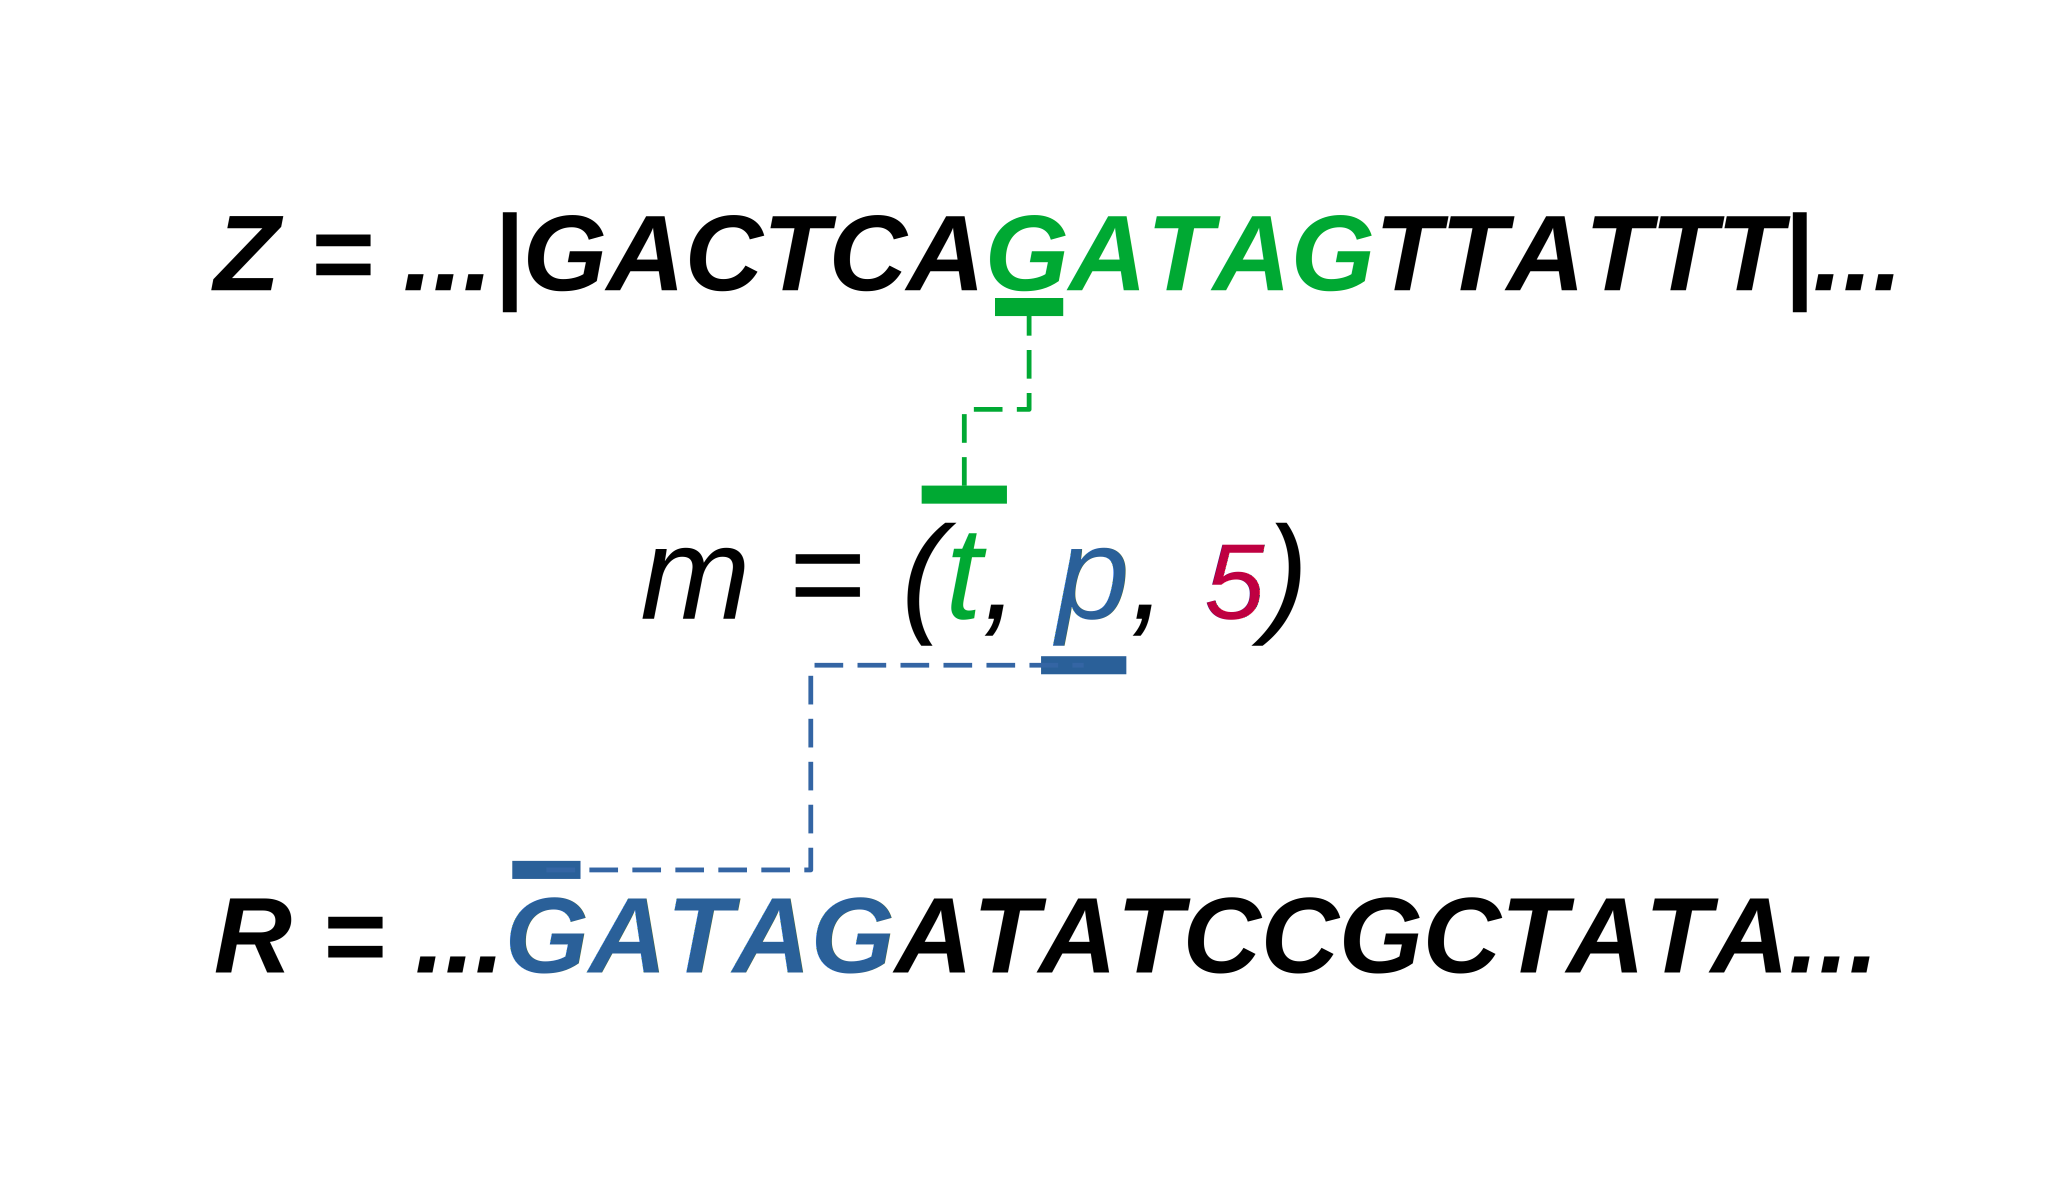
\includegraphics[scale = 0.75]{img/mem.png}
  \caption{Diagramma della struct Mem nel codice originale.}
\end{figure}
Come già detto, l'algoritmo che permette il calcolo degli stessi non è argomento
di questa trattazione ma, per poter usare lo stesso algoritmo sia per il calcolo
dei \textbf{MEMs} tra la read e la linearizzazione dello \textbf{splicing graph}
che tra la read e la linearizzazione delle sequenze introniche, è stato
leggermente modificato il codice dello stesso per poter permettere la produzione
di \textbf{MEMs} differenziati per esoni e introni. A tal fine, la
\textit{struct} è stata modificata aggiungendo semplicemente un valore
\texttt{bool} che, quando posto \texttt{true}, ci segnala che si sta lavorando
su un \textbf{MEM} proveniente dalle sequenze introniche. Parlando, come
anticipato, dell'algoritmo atto al calcolo dei \textbf{MEMs}, chiamato
\textit{backwardMEM}, si segnala che è stato leggermente modificato il codice in
modo da poter stabilire, tramite il costruttore, quale tipologia di \textbf{MEM}
si sta calcolando. 
\begin{figure}
  \centering
  \includegraphics[scale = 0.75]{img/memIntron.png}
  \caption{Diagramma della struct Mem nel codice modificato. Si nota anche
    l'aggiunta dell'overload dell'operatore di uguaglianza al fine di
    riconoscere \textbf{MEMs} uguali e di un metodo di stampa che comprende
    anche la tipologia del \textbf{MEM} stampato.}
  \label{si}
\end{figure}
L'indicazione della tipologia di \textbf{MEM} (figura \ref{si}), specificata
all'interno del 
costruttore della \texttt{struct} (nonché specificato nel costruttore della
classe che si occupa del calcolo dei \textbf{MEMs}), risulterà essenziale per lo
studio del file \texttt{.mem} al fine di verificare l'allineamento con esoni non
annotati in quanto ora il \textbf{MEM} sarà identificato da una quadrupla,
avendo anche la specifica \textit{booleana} della tipologia:
\[m=(t,p,l, intron)\]
\section{Costruzione del MEMs graph}
È stata già descritta precedentemente la struttura del \textbf{MEMs graph} per
cui trattiamo, velocemente, come esso viene costruito.\\
Introduciamo il parametro $L$, di default quantificato in $15$, che rappresenta
la lunghezza minima dei \textbf{MEMs} che verranno calcolati. Una volta ottenuta
tale lista si procede alla creazione del grafo anche se, in realtà, si hanno due
diversi grafi: il cosiddetto \textit{AnnGraph} e il 
\textit{NovGraph}. La particolarità di questo secondo è di tener conto di archi
tra due \textbf{MEMs} indipendentemente dal fatto che sia stato calcolato un
punteggio non compatibile con gli standard imposti a inizio computazione. Dopo
aver calcolato la lista dei \textbf{MEMs} tra la read in analisi e la
linearizzazione si procede analizzando, per ogni \textbf{MEM}, 3 possibili
situazioni:
\begin{enumerate}
  \item si verifica se esso possa essere collegato al nodo iniziale, tramite il
  metodo \texttt{validStart}
  \item si verifica se esso possa essere collegato ad un qualsiasi altro
  \textbf{MEM} della lista, tramite il metodo \texttt{checkMEMs}
  \item si verifica se esso possa essere collegato al nodo finale, tramite il
  metodo \texttt{validEnd} 
\end{enumerate}
Questi tre passaggi possono essere estesi, nel caso dell'\textit{AnnGraph}, per
considerare anche i \textbf{MEMs} provenienti dagli introni, al fine di
ricercare possibili \textit{novel exons}.
\subsection{Lista dei MEMs intronici}
Prima di iniziare a catalogare le varie possibili estensioni è necessario fare
una breve premessa. La cardinalità della lista dei \textbf{MEMs} proveniente
dagli introni è, statisticamente, maggiore, se non molto maggiore, di quella
calcolata sugli esoni. La causa è la lunghezza della linearizzazione e le
motivazioni possono essere riassunte in 2 punti: 
\begin{enumerate}
  \item Una motivazione ``biologica'' causata dall'oggettiva maggior lunghezza
  delle sequenze non codificanti rispetto a quelle codificanti. Questa
  motivazione è visualizzabile nella figura \ref{long}.
  \item Una motivazione ``computazionale'' data dalla scelta di costruire la
  mappa degli introni descritta precedentemente. A causa di quella scelta, si
  avranno sequenze ripetute all'interno della linearizzazione in quanto una
  determinata sequenza non codificante può essere sia riconosciuta come intera
  che eventualmente divisa in più sotto-sequenze. Un esempio può essere
  riscontrato nella figura \ref{img:int}, dove l'introne 3 non è altro che la
  concatenazione degli introni 2, 4 e 5 (comportando che le sequenze relative a
  questi tre possibili introni saranno in realtà già presenti nella
  \textbf{linearizzazione}, implicando delle ripetizioni).
\end{enumerate}
\begin{figure}[H]
  \centering
  \includegraphics[scale = 2.75]{img/ivse.jpg}
  \caption{Visualizzazione di due trascritti dove è possibile notare gli esoni
    (rappresentati mediante rettangoli blu) e gli introni contenuti tra ogni
    coppia di esoni. Si nota come le sequenze introniche siano, statisticamente,
    più lunghe di quelle esoniche.}
  \label{long}
\end{figure}
Avendo a che fare con una lista di \textbf{MEMs} molto estesa si avrà un maggior
carico computazionale in alcuni punti della computazione e a causa di ciò sono
state imposte particolari limitazioni che verranno analizzate.
\subsection{Estensione del MEMs graph esonico}
Una prima situazione in cui possiamo incorrere durante la creazione del
\textbf{MEMs graph} è quella di aver ottenuto una lista di \textbf{MEMs},
proveniente dall'allineamento della read con la linearizzazione degli esoni,
di cardinalità non nulla. Questo fatto ci porta, in primo luogo, a concludere
che sicuramente la read in analisi sarà allineata con uno o più esoni già
annotati e questi allineamenti devono avere la priorità sugli eventuali
allineamenti calcolati sulla linearizzazione degli introni.\\
Un aspetto che non può essere trascurato è quello della selezione degli introni
in cui può essere validato un allineamento. Sempre nell'ottica di dare priorità
agli esoni si è scelto di considerare, eventualmente, solo allineamenti
provenienti da un introne adiacente all'esone considerato (o contenuto in mezzo
a due esoni nel caso in cui si stia valutando un \textit{gap} sulla read,
troppo esteso tra 
due \textbf{MEMs} provenienti da due esoni consecutivi). Inoltre, questa scelta
permette di studiare, in primis, eventuali estensioni di esoni annotati, in
termini di eventi di \textit{alternative acceptor site} e \textit{alternative
  donor site}, con sequenze introniche adiacenti.\\
Abbiamo quindi 3 possibili casi da analizzare, che analizzeremo singolarmente
nel dettaglio:
\begin{enumerate}
  \item Il \textbf{MEM} considerato presenta un valore $p$ maggiore di $L$,
  implicando che un prefisso di read, pari almeno alla lunghezza
  minima su cui sono stati calcolati i \textbf{MEMs}, potrebbe non essere
  allineato con la linearizzazione degli esoni. Inoltre, l'algoritmo originale
  non creerebbe un arco tra il nodo \textit{start} e il nodo del \textbf{MEM}.   
  \item La coppia di \textbf{MEMs} considerata presenta un \textit{gap} sulla
  read, ovvero la distanza tra la fine del primo \textbf{MEM} e l'inizio del
  secondo, maggiore di $L$, implicando 
  che potrebbe esserci una porzione intermedia della read non allineata con la
  linearizzazione degli esoni. Inoltre, l'algoritmo originale
  non creerebbe un arco tra i due nodi relativi ai \textbf{MEMs}.
  \item Il \textbf{MEM} considerato presenta una copertura sulla read terminante
  prima della fine della read stessa, con un margine di lunghezza almeno pari a
  $L$. Questo fatto potrebbe implicare che un suffisso di read potrebbe
  non essere allineato con la linearizzazione degli esoni e il nodo relativo al
  \textbf{MEM} in analisi potrebbe non venir collegato al nodo \textit{end}.
\end{enumerate}
\subsubsection{Estensione iniziale}
È stato già discusso precedentemente quando si necessita di estendere
inizialmente il grafo, discutiamo quindi la modalità. Innanzitutto, vengono
calcolati i \textbf{MEMs} intronici. Una volta calcolati si procede al controllo
dell'introne di provenienza di ogni \textbf{MEM}, infatti, come già discusso,
si studiano solo gli introni adiacenti 
all'esone da cui proviene il \textbf{MEM} che o non risulta essere idoneo per
essere collegato al nodo \textit{start} o risulta essere allineato con la read a
partire da un indice troppo grande. Nel caso dell'estensione iniziale studiamo,
quindi,
l'introne che precede l'esone, ovvero, dato un esone $[b_i,e_i]$, studiamo tutti
gli introni che, nella mappa precedentemente descritta, si trovano contenuti tra
un esone arbitrario $[b,e]$ e l'esone $[b_i,e_i]$, con quest'ultimo posto a
destra rispetto al primo. Vengono quindi selezionati solo i \textbf{MEMs}
validi, 
e vengono calcolate le possibili sequenze (che saranno ordinate secondo il
valore di $p$ in modo crescente) di \textbf{MEMs} valide a colmare il
\textit{gap} iniziale.\\
Si procede quindi, tramite l'uso di \textit{LEMON}, a creare archi tra
\textbf{MEMs} intronici consecutivi in ognuna delle sequenze calcolate. Si
procede poi a collegare, con un arco di peso simbolico pari a 1, l'ultimo nodo
di ogni sequenza al nodo rappresentante il \textbf{MEM} esonico. Infine, si
collega il nodo \textit{start} al primo nodo di ogni sequenza di \textbf{MEMs}
intronici, specificando come peso dell'arco il valore $p$ del nodo 
intronico e segnalando quindi la cardinalità del prefisso di read
eventualmente ancora non allineato di modo che si tenga considerazione della
qualità dell'allineamento stesso in fase di ricerca dei cammini minimi. Quanto
descritto è rappresentato nella figura \ref{in}.
\begin{figure}
  \centering
  \includesvg[scale = 0.6]{img/begvec.svg}
  \caption{Rappresentazione grafica dell'estensione iniziale del \textbf{MEMs
      graph}, con il nodo \textit{start} rappresentato in rosso, i nodi
    rappresentanti i \textbf{MEMs} delle molteplici possibili sequenze
    introniche in verde e il nodo rappresentante il \textbf{MEM} esonico in blu.
    In rosso sono rappresentati gli archi pesati tra il
    nodo \textit{start} e i \textbf{MEMs} intronici.}
  \label{in}
\end{figure}
\subsubsection{Estensione intermedia}
Analizziamo ora la situazione in cui, durante il tentativo di collegare il nodo
relativo al \textbf{MEM} esonico in analisi con un altro \textbf{MEM} esonico
della lista, si trova che il gap sulla read tra questi due \textbf{MEMs} è
superiore a $L$. Si procede, quindi, cercando i \textbf{MEMs} intronici relativi
alle sequenze di introni che, nella mappa precedentemente descritta, presentano
come chiave la coppia di \textit{ID} calcolata tramite \texttt{rank} sui due
\textbf{MEMs} esonici in analisi. Anche in questo caso si ottengono diverse
sequenze di \textbf{MEMs} intronici adeguati e si procede, tramite
\textit{LEMON}, per ogni sequenza, alla creazione di un nodo per ogni
\textbf{MEM} e al collegamento di ogni nodo col successivo, sempre sfruttando
l'ordine basato sul valore $p$ di ogni \textbf{MEM}. Quindi viene collegato il
primo \textbf{MEM} esonico con ogni primo nodo di ogni sequenza, con un arco di
peso simbolico pari a 1, e ogni ultimo nodo di ogni sequenza viene collegato al
nodo del secondo \textbf{MEM}, sempre con un arco di peso pari a 1 di modo che
la ricerca dei cammini minimi veda il percorso con gli introni come un percorso
con ``peso'' maggiore. Quanto descritto è rappresentato nella figura \ref{mid}.
\begin{figure}
  \centering
  \includesvg[scale = 0.6]{img/midvec.svg}
  \caption{Rappresentazione grafica dell'estensione intermedia del \textbf{MEMs
      graph}, con i nodi dei due \textbf{MEMs} esonici rappresentati in blu e i
    nodi rappresentanti i \textbf{MEMs} delle molteplici possibili sequenze
    introniche, che possono colmare il gap sulla read dato dai \textbf{MEMs}, in
    verde.}
  \label{mid}
\end{figure}
\subsubsection{Estensione finale}
Infine, analizziamo l'eventuale estensione finale del \textbf{MEMs
  graph}. Questo accade qualora 
non sia possibile collegare un \textbf{MEM} esonico al nodo \textit{end}, avendo
quindi un suffisso di read di lunghezza maggiore a $L$ non allineato con la
linearizzazione degli esoni. Anche in questo caso, si procede con il calcolo dei
\textbf{MEMs} intronici ritenendo però validi solo quelli provenienti da un
introne posto immediatamente a destra dell'esone studiato. Verranno quindi
utilizzati gli introni di ogni lista, nella mappa precedentemente descritta,
corrispondenti a una chiave dove il primo esone corrisponde all'esone
studiato. Analogamente ai due casi precedenti, si procede a
collegare, per ogni sequenza di \textbf{MEMs} intronici calcolata, tutti i
nodi. Quindi viene collegato, con un arco di peso simbolico pari a 1, il nodo
corrisponde al \textbf{MEM} esonico con il primo nodo di ogni sequenza di
\textbf{MEMs} intronici. Infine, con peso pari alla eventuale lunghezza del
suffisso della read non ancora allineato, si collega l'ultimo nodo di ogni
sequenza con il nodo \textit{end}. Nel dettaglio, tale peso $w$, avendo una read
di lunghezza $l$ e ultimo \textbf{MEM} di una sequenza intronica $m$, è dato da:
\[w = l - (m_p + m_l)\]
Quanto descritto è rappresentato nella figura \ref{end}.
\begin{figure}
  \centering
  \includesvg[scale = 0.6]{img/endvec.svg}
  \caption{Rappresentazione grafica dell'estensione finale del \textbf{MEMs
      graph}, con il nodo rappresentante il \textbf{MEM} esonico in blu, i nodi
    rappresentanti i \textbf{MEMs} delle molteplici possibili sequenze
    introniche in verde e il nodo \textit{end} rappresentato in rosso. Sempre in
  rosso sono rappresentati gli archi pesati tra i \textbf{MEMs} intronici e il
  nodo \textit{end}.}
  \label{end}
\end{figure}
\subsection{Costruzione del MEMs graph intronico}
Fino ad ora abbiamo trattato unicamente il caso in cui la lista dei
\textbf{MEMs} 
esonici non fosse vuota ma non sempre possiamo ottenere questa
situazione. Inoltre, potrebbe anche accadere che non esistano archi, nonostante
il tentativo di estensione, che raggiungano il nodo \textit{end} o che, alla
fine della costruzione partendo dai \textbf{MEMs} esonici si arrivi a un grafo
contenete solo due nodi, il nodo \textit{start} e il nodo \textit{end}. In tal
caso viene costruito il \textbf{MEMs graph} in modo analogo a quanto fatto nel
codice originale in merito alla costruzione del grafo in presenza di soli
\textbf{MEMs} esonici. Si ha però qualche differenza. In primis non si ha la
costruzione del \textit{NovGraph}, ma solo dell'\textit{AnnGraph}, come già
indicato precedentemente nel caso dell'estensione del grafo. Vengono quindi
costruiti tre metodi analoghi ai metodi \texttt{validStart}, \texttt{validEnd} e
\texttt{checkMEMs} che sfruttano i metodi \texttt{rank} e \texttt{select} sugli
introni. A causa della strategia di riconoscimento degli introni, non si avrà un
equivalente dello \textbf{splicing graph} e quindi una lista di nodi
\textit{genitore} e di nodi \textit{figlio} per ogni nodo del grafo ma verrà
sfruttato l'ordine crescente degli introni al fine di sopperire a questa
mancanza.\\
Come anticipato, la lunghezza della linearizzazione degli introni può risultare
 un grosso problema dal punto di vista computazionale. Si consideri di avere
una grossa annotazione, con decine di trascritti ed esoni piccoli e molto
distanti tra loro. A causa della lunghezza degli esoni si otterrà una
linearizzazione molto lunga con una gran quantità di \textbf{MEMs} di piccola
lunghezza (quindi in un intorno del valore $L$). In fase di costruzione del
\textbf{MEMs graph}, in particolare durante il tentativo di studiare i
collegamenti tra un \textbf{MEM} ed un altro appartenente alla lista,
si potrebbe incorrere in computazioni non sostenibili in situazioni ``normali''
nonché spesso inutili. Si procede quindi con una scelta a priori in merito alla
massima lunghezza della linearizzazione degli introni per la quale effettuare
uno studio completo con valore $L$ pari a quella degli esoni. Si è optato, in
via iniziale, per una lunghezza massima pari a 500000 caratteri. Oltre tale
lunghezza, nel caso di calcolo dei \textbf{MEMs} intronici, verrà utilizzato un
nuovo valore di lunghezza minimo pari a metà della lunghezza della read che si
cerca di allineare. A causa di questa scelta, in determinati casi, si potrebbero
avere risultati di qualità peggiore, nonostante gli allineamenti più consistenti
vengano comunque identificati permettendo quindi di identificare, con buona
precisione, eventuali \textit{novel exons}.
\begin{figure}
  \centering
  \includesvg[scale = 0.5]{img/reads4.svg}
  \caption{Rappresentazione grafica dei possibili allineamenti. In alto si hanno
    due esoni annotati, in verde, e un esone non annotato in verde
    chiaro. Si nota che tali esoni sono ordinati nel genoma di
    riferimento. L'esone non annotato è quindi contenuto nell'introne che, a sua
    volta, è posto tra i due esoni annotati, consecutivi tra loro nel
    genoma. Sotto, invece, sono rappresentati diversi allineamenti possibili,
    segnalando in blu gli allineamenti con esoni annotati e in grigio quelli con
    l'esone non 
    annotato. Nel \emph{primo caso} abbiamo una rappresentazione
    dell'\textit{estensione intermedia} tramite un \textbf{MEM} intronico; nel
    \emph{secondo caso} abbiamo una read che ``cade'' sui due esoni annotati;
    nel \emph{terzo caso}, invece, abbiamo un esempio di \textit{estensione
      iniziale} 
    tramite un \textbf{MEM} intronico che permette a un prefisso della read di
    essere allineato (viene esteso il grafo originale che avrebbe calcolato solo
    un allineamento con il secondo esone annotato, non ritenendolo probabilmente
    sufficiente); nel \emph{quarto caso} si ha un esempio di read che ``cade''
    interamente in un esone non annotato (per la quale quindi si procede allo
    studio del solo \textbf{MEMs graph intronico}); nel \emph{quinto caso} si
    ha un esempio di \textit{estensione finale} tramite un \textbf{MEM}
    intronico 
    che permette a un suffisso della read di essere allineato (viene esteso il
    grafo originale che avrebbe calcolato solo un allineamento con il primo
    esone annotato, non ritenendolo probabilmente sufficiente); negli
    \emph{ultimi due casi} si hanno due read che cadono interamente,
    rispettivamente, nel secondo e nel primo esone.}   
\end{figure}
\\Bisogna specificare, inoltre, che allo stato attuale, a causa, in primis, di un
mancato studio approfondito del peso degli archi in presenza di \textbf{MEMs}
intronici, agli allineamenti contenenti introni è permesso un peso massimo
maggiore di quello usato in presenza di soli \textbf{MEMs} esonici.\\
\textit{Tutte le estensioni ad ASGAL fino ad ora introdotte possono essere
  attivate 
  tramite l'opzione \texttt{-i} o l'opzione estesa \texttt{--introns} da
  specificare all'esecuzione dell'eseguibile nominato
  \texttt{SpliceAwareAligner}}.

\section{Ultimi passaggi}
Dopo la ricerca, per ogni read, di ogni allineamento, comprendente anche
eventuali allineamenti con porzioni non codificanti del genoma, avremo i
risultati salvati in un file \texttt{.mem}, la cui struttura è stata già
descritta. Notiamo, però, che in questo caso i singoli \textbf{MEMs} non sono
più rappresentati da una tripla ma da una quadrupla dove il quarto campo
rappresenta la provenienza del \textbf{MEM}. Si avrà quindi il valore $0$ se
proviene da un esone annotato mentre si avrà il valore $1$ se proviene da un
introne. Questa notazione semplificherà l'uso di alcuni scripts che ora verranno
descritti.
\subsection{Creazione del file SAM}
Riprendendo la pipeline di ASGAL notiamo come un primo risultato sia quello di
ottenere un file \textbf{SAM} per rappresentare gli allineamenti. Nel progetto
originale si ha uno script, chiamato \texttt{formatSAM.py}, che, preso in
ingresso il genoma di riferimento, l'annotazione associata e il file
\texttt{.mem} precedentemente costruito, genera il file \textbf{SAM}.\\
Nella realtà l'annotazione serve principalmente per poter risalire al file
\texttt{.sg} con la descrizione dello \textbf{splicing graph} associato al fine
di risalire alle informazioni in esso descritte. \\
Al fine di permettere l'integrazione dei \textbf{MEMs} intronici si sfrutta il
file \texttt{.intron.sg} precedentemente descritto, creando, inoltre, un
\textit{bit vector} (non ottimizzato) per la \textbf{linearizzazione} ottenuta
tramite la concatenazione della \textbf{linearizzazione} intronica a quella
esonica. Si procede, in fase di lettura dei \textbf{MEMs} nello script, a creare
un'unica lista con \textbf{MEMs} esonici e intronici. A tal fine questi ultimi
vengono modificati in modo che il loro valore $t$ possa identificare gli
introni, la cui lista viene posta in fondo alla lista degli esoni. Saputa
quindi la lunghezza della linearizzazione esonica originale, si procede
aggiungendo tale valore a ogni campo $t$ dei \textbf{MEMs} che presentano $1$
come quarto valore (quarto valore che dopo questa procedura non viene più
sfruttato). Si procede quindi con il calcolo originale delle stringhe
\textit{CIGAR}, calcolo che potrà sfruttare l'omogeneizzazione delle due
tipologie di \textbf{MEMs}.\\ 
Una volta prodotto il file \textbf{SAM} verrà sfruttato
\textit{SAMtools} \cite{sam} al fine di produrre il file \textbf{BAM} associato,
utile nello studio dei risultati.
\chapter{Risultati}
Al fine di poter discutere i risultati è bene prima descrivere sommariamente
alcuni strumenti utilizzati a tal fine.
\section{Script per lo studio dei risultati}
Ulteriori scripts sono stati scritti al fine di studiare la qualità dei
risultati e permettere una sperimentazione completa su interi cromosomi. Si ha
quindi una breve anticipazione di tali scripts:
\begin{itemize}
  \item Lo script denominato \texttt{splitGene.py} che, data in ingresso
  un'annotazione completa, separa il singolo file \textbf{GTF} in una serie di
  files \textbf{GTF}, uno per ogni gene.
  \item Lo script denominato \texttt{removeExon.py} che, data in ingresso
  un'annotazione contenente 
  un singolo gene, rimuove, ove possibile, un esone, di lunghezza contenuta in un
  range desiderato, scelto in modo casuale da
  ogni trascritto. La rimozione dell'esone deve comunque garantire che non
  rimanga un solo esone, fattore che, per come è stato impostato lo studio sugli
  introni, renderebbe impossibile lo stesso (avendo scelto di considerare solo
  porzioni di genoma non codificanti contenute tra due porzioni codificanti). Il
  risultato prodotto sarà quindi un'annotazione contenuta in un file
  \textbf{GTF}.
  \item Lo script denominato \texttt{compareMem.py} che, dati in ingresso due
  files \texttt{.mem}, 
  provenienti da due annotazioni (una è il risultato della eventuale
  rimozione di un esone dell'altra), confronta, per ogni read allineata, i due
  allineamenti e produce un semplice file di testo \texttt{.txt} contenente i
  risultati.
  \item Lo script denominato \texttt{generatePlot.py} che, dato in ingresso un
  insieme di files di 
  testo con i risultati ottenuti dall'esecuzione di \\\texttt{compareMem.py}
  genera degli istogrammi, tramite \textit{matplotlib} \cite{matplotlib}, al
  fine di poter visualizzare la qualità degli stessi. Tale script genera anche
  dei files di testo contenenti i risultati numerici.
  \item Lo script denominato \texttt{formatGTF.py} che, dato in ingresso il
  genoma di riferimento, 
  l'annotazione in formato \textbf{GTF} e il file \texttt{.mem}, ricostruisce i
  probabili indici di inizio e fine degli eventuali \textit{novel exons}, al
  fine di poterli eventualmente includere in una nuova annotazione.
\end{itemize}
\section{Analisi dei risultati}
Si descrivono ora i risultati ottenuti. Durante lo sviluppo del progetto ci sono
stati due momenti di analisi dei risultati:
\begin{itemize}
  \item Un primo momento, nei primi 2 mesi e mezzo di progetto, in cui veniva
  studiata una piccola annotazione, con 3 trascritti da 6 o 7 esoni ciascuno,
  relativa al \textit{cromosoma X} umano. A tale annotazione sono
  stati manualmente rimossi 2 esoni non consecutivi (figura \ref{vis}) al fine
  di permettere uno 
  studio più immediato dei risultati man mano ottenuti. Tale genoma e tale
  annotazione possono essere ritrovati nella cartella d'esempio della repository
  di \textit{ASGAL}
  \footnote{\url{https://github.com/AlgoLab/galig/tree/master/example}}.  
  \item Un secondo momento, nelle ultime settimane, in cui lo studio si è
  spostato sugli interi genomi e sulle intere annotazioni di 3 cromosomi umani,
  il \textbf{cromosoma 1} (interessante in quanto risulta essere il più lungo
  cromosoma dell'uomo), il \textbf{cromosoma 9} e il 
  \textbf{cromosoma 21} (uno dei più piccoli cromosomi dell'uomo).
\end{itemize}
Per quanto riguarda l'\textbf{RNA-Seq sample} è stato usato un tool, chiamato
\textit{RNASeqReadSimulator} \cite{seq} \cite{seq2}, che permette di generare un
numero desiderato di reads, di lunghezza ed \textit{error rate} arbitrari, a
partire da un genoma e dall'annotazione associata.
\begin{shaded}
  Durante il test è stata usata una macchina con le seguenti specifiche
  tecniche: 
  \begin{itemize}
    \item processore \textit{Intel Core i7-8550U} con $4$ cores, $8$ threads,
    frequenza base $1.80$GHz e frequenza \textit{Turbo Boost} $4$GHz
    \item ram di quantità pari a $8$Gb
  \end{itemize}
  Il sistema operativo utilizzato è una distribuzione \textit{GNU/Linux}.
\end{shaded}
\subsection{Visualizzazione con IGV}
In questa sezione si introduce l'uso di \textbf{IGV} \cite{igv}, un software,
disponibile sia in versione desktop (scritto in linguaggio \textit{Java}) che in
versione web, atto alla visualizzazione di sequenze genomiche, di annotazioni in
formato \textbf{GTF} e di allineamenti in formato \textbf{BAM}. \\
La visualizzazione tramite \textbf{IGV} è la motivazione principale per cui è
stata implementata la costruzione del file \textbf{SAM} anche a partire dai
\textbf{MEMs} intronici.\\
\begin{figure}
  \centering
  \includegraphics[scale = 0.5]{img/igv.jpg}
  \caption{Visualizzazione tramite IGV delle due annotazioni. Sopra può essere
    osservata l'annotazione originale mentre sotto l'annotazione in cui sono
    stati rimossi i due esoni da ogni trascritto.}
  \label{vis}
\end{figure}
Al fine di poter visualizzare gli allineamenti è stato necessario, tramite
\textit{SAMtools}, generare il file \textbf{BAM} relativo agli stessi e
indicizzarlo (al fine di ottenere un più rapido accesso). Si hanno, a tale
scopo, due semplici comandi \textit{Bash}: 
\begin{verbatim}
samtools view -bS file.sam | samtools sort - > file.bam
samtools index file.bam
\end{verbatim}
Una volta ottenuto il file \textbf{BAM} sono stati confrontati, visivamente,
i risultati. Sono stati analizzati, quindi, due diversi campioni
di \textbf{RNA-Seq sample}. 
\newpage
\subsubsection{Primo sample}
Questo primo campione presenta un \textbf{RNA-Seq sample} con le seguenti
caratteristiche:
\begin{itemize}
  \item lunghezza read: $100$
  \item numero totale di reads: $25000$
  \item error rate: $1\%$
\end{itemize}
Vediamo quindi i risultati ottenuti:
\begin{figure}[H]
  \centering
  \includegraphics[scale = 0.55]{img/igvorig.jpg}
  \caption{Visualizzazione degli allineamenti calcolati tramite \textit{ASGAL}
    originale e annotazione completa.}
  \label{r1}
\end{figure}
\begin{figure}[H]
  \centering
  \includegraphics[scale = 0.55]{img/igvnoe.jpg}
  \caption{Visualizzazione degli allineamenti calcolati tramite \textit{ASGAL}
    originale e annotazione priva dei due esoni. Si può notare la forte perdita
    di allineamenti, rispetto alla precedente figura, nella parte superiore
    dell'immagine.}
  \label{r2}
\end{figure}
\begin{figure}[H]
  \centering
  \includegraphics[scale = 0.55]{img/igvi.jpg}
  \caption{Visualizzazione degli allineamenti calcolati tramite \textit{ASGAL}.
    modificato per allineare con potenziali \textit{novel exons}, e annotazione
    priva dei due esoni. Si può notare in alto come siano stati ``ritrovati''
    gli allineamenti che erano stati persi con la rimozione dei due esoni.}
  \label{r3}
\end{figure}
Si nota, inoltre, che, anche in presenza di un campione di cardinalità ridotta,
composto per di più da reads di piccola dimensione, e di un'annotazione semplice,
con introni non eccessivamente grossi (non a sufficienza da dover rimodulare il
valore $L$), i tempi di esecuzione aumentano di un fattore non trascurabile:
\begin{center}
  \begin{tabular}[c]{c|c}
    \hline
     \cellcolor[gray]{0.6}&  \cellcolor[gray]{0.8}tempo \\
    \hline
    \textit{ASGAL} originale e annotazione completa & $\sim 2.5$s\\
    \hline
    \textit{ASGAL} originale e annotazione modificata & $\sim 2.0$s\\
    \hline
    \textit{ASGAL} con parametro \texttt{--intron}
    e annotazione modificata & $\sim 4.0$s   \\
    \hline
  \end{tabular}
\end{center}
\subsubsection{Secondo Sample}
Il secondo campione presenta un \textbf{RNA-Seq sample} con le seguenti
caratteristiche:
\begin{itemize}
  \item lunghezza read: $300$
  \item numero totale di reads: $100000$
  \item error rate: $1\%$
\end{itemize}
\textbf{\textit{In questo caso verranno omesse le immagini in quanto analoghe a
    quelle del primo sample.}}\\
Si annota che all'aumentare della quantità di read, nonché della loro lunghezza,
anche in presenza di un'annotazione ``semplice'', le differenze dei tempi di
esecuzione iniziano a essere importanti: 
\begin{center}
  \begin{tabular}{c|c}
     \cellcolor[gray]{0.6}&  \cellcolor[gray]{0.8}tempo \\
    \hline
    \textit{ASGAL} originale e annotazione completa & $\sim 34.5$s\\
    \hline
    \textit{ASGAL} originale e annotazione modificata & $\sim 31.5$s\\
    \hline
    \textit{ASGAL} con parametro \texttt{--intron}
    e annotazione modificata & $\sim 55.5$s 
  \end{tabular}
\end{center}
\textit{Possiamo comunque concludere che le reads di entrambi i samples vengono
  allineate, con buona qualità, ai due esoni rimossi, che vengono quindi
  riconosciuti come \emph{novel exons}. Tale qualità verrà
  dimostrata durante la sperimentazione della \emph{seconda fase} nonché con
  l'esecuzione di un piccolo script, atto a una parziale ricostruzione del file
  \textbf{GTF}. La sperimentazione, purtroppo, mostrerà anche come i tempi di
  calcolo saranno anche superiori al ``triplo''  nel momento in cui verranno
  ricercati i \emph{novel exons}.}
\subsubsection{Ricostruzione dell'annotazione}
Come descritto, in questo primo studio, sono stati rimossi due esoni. Il primo
risultava compreso tra gli indici $286949$ e $287041$ mentre il secondo tra gli
indici $289041$ e $289272$. Lo script è in realtà molto semplice, nonché poco
ottimizzato, e si basa su una lista booleana, interamente inizializzata a $0$ di
lunghezza pari alla distanza tra l'indice d'inizio dell'ultimo esone annotato e
l'indice di fine del primo esone annotato (dopo aver ordinato gli esoni in
ordine crescente basandosi sull'indice di partenza). Sfruttando unicamente i
\textbf{MEMs} intronici, quindi con quarto campo pari a $1$, la lista delle
sequenze introniche, la loro linearizzazione (su cui si costruisce un
\textit{bit vector} non ottimizzato), queste ultime contenute nel file
\texttt{.intron.sg}, e le operazioni di \texttt{rank} e \texttt{select}, si
procede a invertire, nella lista booleana, i valori contenuti nelle sequenze di
indici individuate dai \textbf{MEMs} intronici. Infine, dopo un'adeguata
sistemazione degli indici basata sulla posizione della lista booleana nei
confronti del genoma considerato, si procede identificando le sequenze di $1$
come \textit{novel exons}. L'esecuzione sui \textbf{MEMs} calcolati in questa
prima parte di studio dei risultati producono 3 potenziali \textit{novel exons}:
\begin{enumerate}
  \item un primo di indici: $[286946,\,287044]$
  \item un secondo di indici: $[289039,\,289273]$
  \item un terzo di indici: $[289870,\,289885]$
\end{enumerate}
Questo è un ulteriore risultato incoraggiante in quanto i primi due
\textit{novel exons} risultano includere nei loro indici i due esoni rimossi,
con un minimo margine di differenza, mentre il terzo, piccolissimo,
\textit{novel exon}, corrisponde all'inizio del piccolo esone presente solo nel
terzo trascritto (figura \ref{vis}).
\subsection{Sperimentazione mediante Snakemake}
Durante il \textit{secondo momento} si è deciso di procedere con una vera e
propria sperimentazione, al fine di studiare i risultati su interi cromosomi
umani e valutarne, in modo più oggettivo rispetto al semplice riscontro visuale
con IGV, i risultati. Per gestire questa sperimentazione, come già anticipato,
si è deciso di utilizzare \textit{Snakemake}, precedentemente
introdotto. \textit{Snakemake} basa il suo funzionamento sulla costruzione di un
\textbf{DAG (\textit{Directed Acyclic Graph})}, delle regole ma anche
dei singoli \textit{job}, e sul suo studio
al fine di eseguire le regole (eventualmente in modo parallelo) per ottenere un
determinato output. In generale \textit{Snakemake} prende spunto dal
``paradigma'' di \textbf{GNU Make} \cite{make}.
\subsubsection{Pipeline della sperimentazione}
Innanzitutto, all'interno di un file chiamato \texttt{config.yaml} abbiamo
specificato le seguenti informazioni, facilmente modificabili dall'utente al
fine di permettere variazioni sulla sperimentazione senza effettivamente
modificare manualmente la stessa:
\begin{itemize}
  \item il nome della cartella in cui verranno inseriti tutti i files necessari
  alla sperimentazione
  \item il nome di tre diverse sottocartelle della cartella sopra definita, una
  per i dati riguardanti le annotazioni complete, una per  i dati riguardanti le
  annotazioni eventualmente prive di un esone e una per i risultati
  \item l'\textit{url} per poter scaricare il genoma corrispondente a un
  cromosoma 
  \item l'\textit{url} per poter scaricare l'annotazione completa
  \item il nome, specificato o dal numero o dalla lettera, del cromosoma da
  studiare, in modo da poter estrarre dall'annotazione completa quella relativa
  al cromosoma di interesse
  \item la lunghezza minima e la lunghezza massima dell'esone che eventualmente
  si cercherà di rimuovere da ogni annotazione
  \item il numero di reads dell'\textbf{RNA-Seq sample} e la lunghezza delle
  stesse  
\end{itemize}
Si hanno quindi diverse regole, visualizzate nel \textbf{DAG} in figura
\ref{rul}: 
\begin{itemize}
  \item Un primo insieme di regole che scaricano il genoma del cromosoma scelto
  e l'annotazione (da cui viene estratta l'annotazione relativa al cromosoma
  d'interesse). Le due regole di download saranno i due nodi \textit{iniziali}. 
  \item Una regola atta alla divisione dell'annotazione del cromosoma
  d'interesse in tante diverse annotazioni, una per ogni gene. A questo punto
  della 
  sperimentazione bisogna necessariamente introdurre una particolare categoria
  di regole, dette \textit{regole checkpoint}. Tali regole permettono di
  ridefinire lo studio del \textbf{DAG} dopo la corretta esecuzione di una
  determinata regola. Nel nostro caso, prima dell'ottenimento di tutte le
  annotazioni relative ad ogni singolo gene, non avremmo potuto conoscere i nomi
  dei files su cui effettuare la costruzione delle annotazioni con 
  l'esone rimosso, il calcolo dei \texttt{.mem} e l'elaborazione dei
  risultati. Definendo quindi tale regola come \textit{checkpoint} possiamo
  ridefinire il risultato finale che si vuole ottenere sfruttando i nomi dei
  files prodotti dalla regola stessa, che verranno usati come \textit{wildcards}
  per tutta la successiva esecuzione della sperimentazione. A tal fine viene
  quindi utilizzata la funzione \texttt{expand} per ottenere una lista
  contenente tutti i nomi dei files che saranno necessari per completare la
  sperimentazione (nel dettaglio sarà sufficiente specificare i files contenenti
  i risultati finali della stessa in quanto sarà \textit{Snakemake} stesso a
  occuparsi di automatizzare la procedura per ottenerli).
  \item Una regola che si occupa di generare le annotazioni eventualmente prive
  di un esone e porle nella cartella specificata nel file\texttt{.yaml}. Qualora
  non sia possibile rimuovere alcun esone in tale cartella viene posta una copia
  dell'annotazione originale, con nome però modificato, affinché le wildcards
  possano funzionare ugualmente senza ulteriori specifiche alla pipeline. 
  \item Una regola che, partendo da ogni annotazione originale, crea, secondo le
  specifiche definite dall'utente, un \textbf{RNA-Seq sample}. Tale insieme di
  reads verrà utilizzato per tutti i 3 possibili calcoli di \textbf{MEMs},
  quello sull'annotazione originale con \textit{ASGAL} originale, quello
  sull'annotazione modificata con \textit{ASGAL} originale e 
  quello sull'annotazione modificata con \textit{ASGAL} con l'opzione
  \texttt{--intron}.
  \item Tre regole che producono effettivamente i files
  \texttt{.mem} per ognuna delle situazioni sopra descritte. In queste regole
  viene usata un'altra particolare \textit{keyword} offerta da
  \textit{Snakemake}: \textit{benchmark}. Specificando tale \textit{keyword},
  nonché un
  percorso dove salvare, per ogni esecuzione della regola stessa, i risultati in
  un file in formato \textbf{TSV (\textit{Tab-Separated Values})}, % \cite{tsv}
  si può tenere traccia di: 
  \begin{itemize}
    \item informazioni sul tempo di esecuzione
    \item informazioni sull'uso di memoria
    \item informazioni sul carico di \textit{input} e \textit{output}
  \end{itemize}
  Le informazioni relative al tempo di esecuzione e alla quantità di memoria
  utilizzata verranno utilizzate per studiare i risultati della sperimentazione.
  \item Due regole per utilizzare \texttt{compareMem.py} al fine di comparare,
  per ogni annotazione, i files \texttt{.mem} calcolati con \textit{ASGAL}
  originale e 
  annotazione completa con quelli calcolati, mediante \textit{ASGAL} originale e
  \textit{ASGAL} con l'opzione di ricerca sugli introni, sull'annotazione
  eventualmente priva di un esone.
  \item Una regola per utilizzare \texttt{generatePlot.py} al fine di produrre
  gli istogrammi relativi alle differenze di performances e di risultati ottenuti
  con il calcolo delle tre tipologie di files \texttt{.mem}. Tale regola fornisce
  anche risultati testuali salvati in appositi files \texttt{.txt}.
  \item Una regola, definibile come \textit{finale}, che
  specifica, ponendoli come \textit{input}, i files che vogliono essere generati
  come passo finale della pipeline (ovvero i files contenenti i risultati
  numerici e le immagini relative agli istogrammi). Specificando solo l'input
  \textit{Snakemake} orchestrerà l'esecuzione delle regole in modo da poter
  permettere l'esecuzione di quest'ultima, cosa che può accadere sse tali files
  sono stati effettivamente generati. Tale regola, chiamata
  \texttt{run\_after\_checkpoint} in quanto definita dopo la regola checkpoint
  sopra descritta, sarà il \textit{nodo terminante} del \textbf{DAG}.
\end{itemize}
Dal punto di vista del calcolo parallelo \textit{Snakemake} ci offre l'opzione
\texttt{--cores} che ci permette di specificare il numero di cores (anche non
fisici) da dedicare alla pipeline. Ogni \textit{job} verrà eseguito da un core
diverso in modo del tutto automatico. 
\begin{figure}
  \centering
  \includegraphics[scale = 0.55]{img/graph.jpg}
  \caption{\textbf{DAG} delle regole di \textit{Snakemake}. Si specifica che
    tale \textbf{DAG} non è il \textbf{DAG} ottenibile usando l'opzione
    \texttt{--rulegraph} in quanto le regole relative al download e alla
    lavorazione iniziale delle 
    annotazioni non verrebbero mostrate, per la regola
    checkpoint. Il \textbf{DAG} è stato, quindi, adeguatamente esteso al fine
    di poter visualizzare anche tali regole. Possiamo notare
    come si abbia in primis il download dei files necessari con le regole
    \texttt{downloadGenome} e \texttt{downloadAnnotation} (a cui seguono le
    regole \texttt{fetch\_annotation} e \texttt{splitAnnotation} per produrre le
    singole annotazioni). I risultati del download sono necessari per
    generare i vari \textbf{RNA-Seq sample} (tramite la regola
    \texttt{generateReads}), le annotazioni modificate (tramite la regola
    \texttt{removeExon}) e i vari \textbf{MEMs} (essendo necessari, per
    eseguire \textit{ASGAL}, un genoma e un'annotazione). Si hanno poi le regole
    per la comparazione dei \textbf{MEMs} che, necessitando sia dei
    \textbf{MEMs} che delle annotazioni, sono collegate di conseguenza alle
    altre regole. Si ha infine la regola \texttt{generatePlot} che raccoglie i 
    risultati e produce i files richiesti dall'input di
    \texttt{run\_after\_checkpoint}.}
  \label{rul}
\end{figure}
\subsection{Confronto della qualità dei risultati}
Passiamo ora allo studio definitivo dei risultati. Lo script
\texttt{compareMem.py} studia i files \texttt{.mem} e tiene conto,
in una prima analisi che poi verrà approfondita, due situazioni:
\begin{enumerate}
  \item Situazioni di \textit{match} dove i due insiemi di \textbf{MEMs}
  identificati sono i medesimi o dove comunque non si ha perdita di reads.
  \item Situazioni di \textit{mismatch} dove non si ha uno dei due insiemi di
  \textbf{MEMs} per una certa read (che non viene quindi allineata in uno dei
  due studi).
\end{enumerate}
Si ha, quindi, una seconda verifica, anche se ancora non molto dettagliata,
della bontà dei risultati ottenuti.\\
Vengono quindi generati dei semplici istogrammi con 3 colonne:
\begin{enumerate}
  \item In \textbf{verde} i dati relativi ad \textit{ASGAL} originale con
  annotazione non modificata. Tali valori saranno, in ogni istogramma, da
  considerarsi come il \textit{valore ideale}.
  \item In \textbf{giallo} i dati relativi ad \textit{ASGAL} con l'opzione
  \texttt{--intron} e con annotazione eventualmente priva di esone. Tali valori
  corrispondono ai risultati a cui si è giunti con la ricerca di \textit{novel
    exons} all'interno di sequenze ritenute non codificanti.
  \item In \textbf{rosso} i dati relativi ad \textit{ASGAL} originale con
  annotazione eventualmente priva di un esone. Tale dato ci conferma che
  effettivamente c'è stata, all'interno dell'intera sperimentazione su ogni
  cromosoma, un'effettiva rimozione di esoni in quanto \textit{ASGAL} non riesce
  più a ottenere gli allineamenti ottenuti originariamente.
\end{enumerate}
Analizzando l'istogramma (figura \ref{data}) troviamo 3 blocchi:
\begin{enumerate}
  \item le colonne rappresentanti la media dei \textit{match}
  \item le colonne rappresentanti la media dei \textit{mismatch}
  \item una verifica sul numero totale delle reads, al fine di avere un
  riscontro sulla bontà dei conteggi
\end{enumerate}

\begin{figure}
  \centering
  \includegraphics[scale = 0.65]{img/data1.png}
  \caption{Esempio di istogramma relativo allo studio dei risultati sul
    cromosoma 1 con \textit{error rate} pari all'$1\%$.}
  \label{data}
\end{figure}
\begin{comment}
  \begin{figure}
    \centering
    \includegraphics[scale = 0.65]{img/data21.png}
    \caption{Istogramma relativo allo studio dei risultati sul ventunesimo
      cromosoma con \textit{error rate} pari all'$1\%$}
  \end{figure}
  \begin{figure}
    \centering
    \includegraphics[scale = 0.35]{img/data9.png} 
    \centering
    \includegraphics[scale = 0.35]{img/data91.png}
    \caption{Esempio di istogramma relativo allo studio dei risultati sul nono
      cromosoma con \textit{error rate} pari all'$1\%$ a sinistra e al $2\%$ a
      destra. Un tale cambiamento di \textit{error rate} usato per simulare
      l'\textbf{RNA-Seq sample} non influisce significativamente la qualità dei
      risultati}  
  \end{figure}
\end{comment}
Si segnala, fin da ora, come dal punto di vista dei risultati non si abbiano
sostanziali differenze, nonostante verranno in seguito analizzati risultati più
approfonditi. La media degli insiemi di \textbf{MEMs} persi risulta 
praticamente nulla se comparata al numero totale di reads mentre, di contro, i
match perfetti e quelli con un certo errore sono elevati. È stato verificato,
inoltre, che la scelta di favorire le performances, aumentando il valore del
parametro $L$ in presenza di una linearizzazione intronica troppo estesa,
perlomeno da un punto di vista statistico, non influisce sulla qualità dei
risultati in quanto si potrà notare dalle tabelle a fine sezione, dove verrà
conclusa l'analisi dei risultati, come la maggior parte delle
reads vengono allineate. Un discorso analogo può essere fatto in merito al
cambiamento di \textit{error rate}.\\
Si riscontra come anche lo studio di diversi cromosomi produce risultati
statisticamente paragonabili, come del resto ci si poteva attendere.
L'unica differenza tangibile tra le diverse sperimentazioni è la quantità di
geni presenti nelle annotazioni complete, che risulterà nel numero di files
\textbf{GTF} da analizzare. Si ha infatti che: 
\begin{itemize}
  \item il \textit{cromosoma 1} conta $5475$ geni (e quindi differenti files
  \textbf{GTF})
  \item il \textit{cromosoma 9} conta $2333$ geni
  \item il \textit{cromosoma 21} conta solo $875$ geni 
\end{itemize}
\section{Confronto delle performances}
Nonostante la qualità dei risultati della sperimentazione risulti essere
parecchio incoraggiante non si può dire altrettanto delle performances, in
primis dal punto di vista dei \textit{tempi di esecuzione}.
\subsubsection{Uso medio della memoria}
In merito all'uso della memoria non si hanno particolari comportamenti da
segnalare in 
quanto i valori delle varie esecuzioni sono comparabili sia a parità di
\textit{error rate} che al variare dello stesso. Si segnala, nel caso del
\textit{cromosoma 9}, un calo dell'uso della memoria all'aumentare
dell'\textit{error rate}, ma non si hanno evidenze del fatto che sia un
miglioramento intrinseco o di altra natura. Un esempio di istogramma
relativo all'uso medio di memoria è visualizzabile nella figura
\ref{img:ista}

\begin{figure}
  \begin{subfigure}{.5\textwidth}
    \centering
    \includegraphics[scale = 0.39]{img/mems1.png}
    \caption{}
    \label{img:ista}
  \end{subfigure}
  \begin{subfigure}{.5\textwidth}
    \centering
    \includegraphics[scale = 0.39]{img/times1.png}
    \caption{}
    \label{img:istb}
  \end{subfigure}
   \caption{Esempio di istogrammi relativi allo studio dell'uso medio della
    memoria (espresso in \emph{Mb}), nella figura \ref{img:ista}, e del tempo
    medio (espresso in \emph{s}), nella figura \ref{img:istb}, registrati
    durante la sperimentazione effettuata sul\emph{ cromosoma 1} con
    \textit{error rate} pari all'$1\%$.}
  \label{perf}
\end{figure}




\begin{comment}
  \begin{figure}
    \centering
    \includegraphics[scale = 0.35]{img/mems9.png} 
    \centering
    \includegraphics[scale = 0.35]{img/mems91.png}
    \caption{Istogramma relativo allo studio dell'uso medio della memoria sul
      nono 
      cromosoma con \textit{error rate} pari all'$1\%$ a sinistra e al $2\%$ a
      destra.}  
  \end{figure}
  \begin{figure}
    \centering
    \includegraphics[scale = 0.65]{img/mems21.png}
    \caption{Istogramma relativo allo studio dell'uso medio della memoria sul
      ventunesimo cromosoma con \textit{error rate} pari all'$1\%$.}  
  \end{figure}
\end{comment}

\subsubsection{Tempo medio di esecuzione}
Analizzando il tempo di esecuzione medio della ricerca dei \textbf{MEMs} si
segnala che la simulazione, prima dell'introduzione della modifica sulla
lunghezza minima dei \textbf{MEMs} intronici in presenza di linearizzazioni
introniche troppo lunghe, non riusciva, sulla macchina di test,
a essere portata a conclusione a causa di interruzioni imposte dal sistema
operativo a loro volta causate da \textit{jobs} che, dopo lunghe attese di tempo
(nell'ordine 
di diverse ore), non
riuscivano a essere conclusi, da qui la necessità di introdurre tale
ottimizzazione. Si riscontra, inoltre, che la modifica di \textit{error rate}
non influisce in modo rilevante sui tempi di esecuzione. Si noterà comunque dai
dati che i tempi medi con la ricerca di \textit{novel exons}, sull'annotazione
priva di un esone, incrementeranno all'aumentare della grandezza del genoma e
all'aumentare del numero di geni, arrivando, nel caso del \textit{cromosoma 1},
a essere oltre il triplo dei tempi originali, probabilmente a causa di singole
annotazioni geniche particolarmente complesse. Un esempio di istogramma
relativo ai tempi medi d'esecuzione è visualizzabile nella figura
\ref{img:istb}. 

% \begin{figure}
%   \centering
%   \includegraphics[scale = 0.65]{img/times1.png}
%   \caption{Esempio di istogramma relativo allo studio del tempo medio di
%     esecuzione del calcolo dei \textbf{MEMs} sul cromosoma 1}  
%   \end{figure}
\begin{comment}
  \begin{figure}
    \centering
    \includegraphics[scale = 0.35]{img/times9.png} 
    \centering
    \includegraphics[scale = 0.35]{img/times91.png}
    \caption{Istogramma relativo allo studio del tempo medio di esecuzione del
      calcolo dei \textbf{MEMs} sul nono cromosoma con \textit{error rate} pari
      all'$1\%$ a sinistra e al $2\%$ a destra}  
  \end{figure}
  \begin{figure}
    \centering
    \includegraphics[scale = 0.65]{img/times21.png}
    \caption{Istogramma relativo allo studio del tempo medio di esecuzione del
      calcolo dei \textbf{MEMs} sul ventunesimo cromosoma con \textit{error rate}
      pari all'$1\%$}   
  \end{figure}
\end{comment}
\subsection{Tabelle riassuntive dei risultati}
Vediamo quindi, più nel dettaglio, le tabelle dei risultati ottenuti sulle 4
sperimentazioni.\\
La prima tabella rappresenta i dati dell'esecuzione di ASGAL sull'annotazione
originale. Sono quindi riportati, per ogni riga, i diversi cromosomi con
l'\textit{error rate} (\textit{e.r}) usato per la generazione delle reads. Si
hanno poi le colonne relative al tempo medio d'esecuzione e alla memoria media
usata per il calcolo degli allineamenti.\\
Passando alla tabella relativa alle esecuzioni sull'annotazione modificata si
hanno le righe dedicate ai vari cromosomi, con l'\textit{error rate}
(\textit{e.r.}) associato, e ognuna di queste righe è a sua 
volta divisa in due, differenziando i due \textit{tipi} di esecuzione:
\begin{enumerate}
  \item La prima riga con i risultati dell'esecuzione di ASGAL con l'opzione
  \texttt{--intron} sull'annotazione modificata. Nominiamo tale riga
  \textit{intron}.
  \item La seconda riga con i risultati dell'esecuzione di ASGAL senza l'opzione
  \texttt{--intron} sull'annotazione modificata. Nominiamo tale riga
  \textit{noIntron}. Tale riga è necessaria per valutare l'effettiva rimozione di
  un esone in modo da poter correttamente analizzare i dati delle
  sperimentazioni.
\end{enumerate}
Per quanto riguarda le colonne della tabella riportante i risultati ottenuti con
l'annotazione modificata si hanno: 
\begin{enumerate}
  \item I \textit{match}, ovvero quante reads mediamente allineano le medesime
  sequenze genomiche rispetto all'esecuzione di ASGAL sull'annotazione
  originale. La colonna viene nominata \textit{match}.
  \item I \textit{semi-match}, ovvero quante reads mediamente allineano
  sequenze genomiche al più di un $10\%$ della lunghezza della read rispetto
  all'esecuzione di ASGAL sull'annotazione originale (quindi con errore
  inferiore al $10\%$ della lunghezza della read). In altri termini si parla
  dei casi in cui una read effettivamente allinea in entrambi gli studi e
  la differenza di copertura tra i due allineamenti è accettabile. La colonna
  viene nominata \textit{$\leq$10\%}. 
  \item I \textit{semi-mismatch}, ovvero quante reads mediamente allineano
  sequenze genomiche oltre al $10\%$ della lunghezza della read rispetto
  all'esecuzione di ASGAL sull'annotazione originale (quindi con errore
  superiore al $10\%$ della lunghezza della read). In altri termini si parla
  dei casi in cui una read effettivamente allinea in entrambi gli studi, ma
  la differenza di copertura tra i due allineamenti è eccessiva. La colonna
  viene nominata \textit{$>$10\%}.
  \item I \textit{mismatch}, in altre parole qualsiasi situazione diversa da
  quelle 
  precedentemente descritte, ovvero, in primis, quante reads 
  risultano allineate solo in una delle due esecuzioni, quella in studio o
  quella con ASGAL sull'annotazione originale. A tal
  proposito si segnala come potrebbero esserci reads allineate solo nel caso di
  studio degli introni a causa dell'aumento del massimo peso accettabile durante
  la ricerca del cammino minimo, fattore che comporterebbe un
  \textit{mismatch}. La 
  colonna viene nominata \textit{mismatch}.
  \item Il tempo medio di esecuzione. La colonna viene nominata \textit{tempo}.
  \item La memoria media utilizzata. La colonna viene nominata \textit{RAM}.
\end{enumerate}
\textit{Si segnala che, in caso di mancata rimozione dell'esone si potrebbero
  avere comunque files \texttt{.mem} (in ogni caso molto pochi) diversi tra
  l'esecuzione originale di ASGAL e quella con l'opzione \texttt{--intron} in
  quanto viene aumentato il massimo peso accettabile durante la ricerca del
  cammino minimo.}\\ 
\textit{Si ricorda, inoltre, che tutti i dati sono stati calcolati partendo da
  un \textbf{RNA-Seq sample} di 25000 reads lunghe 100. Per tutte le
  sperimentazioni è stata usata l'opzione \texttt{--cores 4} per quanto riguarda
  \emph{Snakemake}.}\\
\\
\begin{comment}
  \textbf{Tabella relativa al cromosoma 1 con \textit{error rate} pari al
    $1\%$. La sperimentazione di ASGAL con annotazione completa ha riportato un
    tempo medio pari a $4.6$s ed un uso medio di RAM pari a $139.3$Mb:}
\begin{center}
  \begin{tabular}{c||c|c|c|c|c|c}
    & match & semi-match & semi-mismatch & mismatch & tempo & RAM\\
    \hline
    \hline
    intron & 24727 & 212 & 29 & 32 & 14.9s & 148.7Mb\\
    \hline
    noIntron & 23026 & 75 & 7 & 1892 & 4.4s & 139.1Mb
  \end{tabular}
\end{center}
 \textbf{Tabella relativa al cromosoma 9 con \textit{error rate} pari al
    $1\%$. La sperimentazione di ASGAL con annotazione completa ha riportato un
    tempo medio pari a $4.7$s ed un uso medio di RAM pari a $55.4$Mb:} 
\begin{center}
  \begin{tabular}{c||c|c|c|c|c|c}
    & match & semi-match & semi-mismatch & mismatch & tempo & RAM\\
    \hline
    \hline
    intron & 24747 & 194 & 23 & 36 & 9.6s & 59.1Mb\\
    \hline
    noIntron & 22993 & 64 & 6 & 1937 & 4.6s & 57.2Mb
  \end{tabular}
\end{center}
\textbf{Tabella relativa al cromosoma 9 con \textit{error rate} pari al
  $2\%$. La sperimentazione di ASGAL con annotazione completa ha riportato un
  tempo medio pari a $4.7$s ed un uso medio di RAM pari a $59.1$Mb:} 
\begin{center}
  \begin{tabular}{c||c|c|c|c|c|c}
    & match & semi-match & semi-mismatch & mismatch & tempo & RAM\\
    \hline
    \hline
    intron & 24748 & 194 & 23 & 35 & 9.6s & 59.2Mb\\
    \hline
    noIntron & 22993 & 64 & 6 & 1937 & 4.6s & 57.9Mb
  \end{tabular}
\end{center}
\textbf{Tabella relativa al cromosoma 9 con \textit{error rate} pari al
  $10\%$. La sperimentazione di ASGAL con annotazione completa ha riportato un
  tempo medio pari a $4.7$s ed un uso medio di RAM pari a $47.7$Mb:}
\begin{center}
  \begin{tabular}{c||c|c|c|c|c|c}
    & match & semi-match & semi-mismatch & mismatch & tempo & RAM\\
    \hline
    \hline
    intron & 24748 & 193 & 23 & 36 & 10.0s & 49.7Mb\\
    \hline
    noIntron & 22991 & 64 & 6 & 1939 & 4.6s & 49.5Mb
  \end{tabular}
\end{center}

\textit{Si può quindi notare come il cambiamento di \emph{error rate} non
  comporti praticamente alcune differenza nella media dei risultati.\\}
\textbf{Tabella relativa al cromosoma 21 con \textit{error rate} pari al
  $1\%$. La sperimentazione di ASGAL con annotazione completa ha riportato un
  tempo medio pari a $4.2$s ed un uso medio di RAM pari a $29.7$Mb:}
\begin{center}
  \begin{tabular}{c||c|c|c|c|c|c}
    & match & semi-match & semi-mismatch & mismatch & tempo & RAM\\
    \hline
    \hline
    intron & 24732 & 220 & 26  & 22 & 8.1s & 30.6Mb \\
    \hline
    noIntron & 22750 & 85 & 9 & 2156 & 3.9s & 29.7Mb
  \end{tabular}
\end{center}
\end{comment}
Abbiamo quindi la tabella relativa all'esecuzione originale, tali valori medi
possono essere visti come il risultato ideale. Si nota come idealmente ci si
aspettino 25000 allineamenti, ma annotazioni estremamente
piccole, con un solo esone, non permettono neppure di poter generare le reads,
comportando, di fatto, files \texttt{.fa} e \texttt{.mem} vuoti. Nel dettaglio,
nelle sperimentazioni effettuate, si ha che:
\begin{itemize}
  \item Per il \texttt{cromosoma 1}, che conta 5465 geni, si hanno 278
  annotazioni che comportano risultati nulli nel caso di generazione
  delle reads con \textit{error rate} pari al 1\%.
  \item Per il \texttt{cromosoma 9}, che conta 2333 geni, si hanno:
  \begin{itemize}
    \item 137 annotazioni che comportano risultati nulli nel caso di generazione
    delle reads con \textit{error rate} pari al 1\%.
    \item 119 annotazioni che comportano risultati nulli nel caso di generazione
    delle reads con \textit{error rate} pari al 2\%.
    \item 118 annotazioni che comportano risultati nulli nel caso di generazione
    delle reads con \textit{error rate} pari al 10\%.
  \end{itemize} 
  \item Per il \texttt{cromosoma 21}, che conta 875 geni, si hanno 44
  annotazioni che comportano risultati nulli nel caso di generazione
  delle reads con \textit{error rate} pari al 1\%.
\end{itemize}
\textit{Quindi circa il 5\% delle annotazioni di ogni cromosoma non permette la
  generazione di un \textbf{RNA-Seq Sample} con il metodo adottato nel
  progetto.}
\\  
Passiamo quindi alla tabella delle \textit{performances medie ideali} (ottenute
con l'esecuzione originale di ASGAL su ogni annotazione non modificata):
\begin{center}

  \begin{tabular}{c|c|c}
    \hline
    \cellcolor[gray]{0.6}& \cellcolor[gray]{0.8}tempo & \cellcolor[gray]{0.8}RAM\\

    \hline
    cromosoma 1, e.r=1\% & 4.6s & 139.3Mb\\
    \hline
    cromosoma 9, e.r=1\% & 4.7s & 55.4Mb\\
    \hline
    cromosoma 9, e.r=2\% & 4.7s & 59.1Mb\\
    \hline
    cromosoma 9, e.r=10\% & 4.7s & 47.7Mb\\
    \hline
    cromosoma 21, e.r=1\% & 4.2s & 29.7Mb\\
    \hline
  \end{tabular}
\end{center}

Passiamo quindi alla tabella con i dati medi relativi all'esecuzione, sempre con
un \textbf{RNA-Seq sample} da 25000 reads (lunghe 100) per gene, di ASGAL
originale e con l'opzione \texttt{--intron} su annotazioni alle quali è stato
eventualmente rimosso un esone:   

\begin{center}
  \resizebox{\textwidth}{!}{%
    \begin{tabular}{c|c|c|c|c|c|c|c}
      \hline
      \cellcolor[gray]{0.6}& \cellcolor[gray]{0.8}tipo &\cellcolor[gray]{0.8} match & \cellcolor[gray]{0.8}$\leq$10\% & \cellcolor[gray]{0.8}$>$10\% & \cellcolor[gray]{0.8}mismatch &\cellcolor[gray]{0.8} tempo & \cellcolor[gray]{0.8}RAM\\
      
      \hline
      \multirow{2}{5em}{\small{cromosoma 1, e.r.=1\%}} & intron & 24727 & 212 & 29 &
                                                                                     32
                                                                                                                                                                                     & 14.9s & 148.7Mb\\
                           &noIntron & 23026 & 75 & 7 & 1892 & 4.4s & 139.1Mb\\
      \hline
      \multirow{2}{5em}{\small{cromosoma 9, e.r.=1\%}} & intron & 24747 & 194 & 23 & 36 & 9.6s & 59.1Mb\\
                           & noIntron & 22993 & 64 & 6 & 1937 & 4.6s & 57.2Mb\\
      \hline
      \multirow{2}{5em}{\small{cromosoma 9, e.r.=2\%}} & intron & 24748 & 194 & 23 & 35 & 9.6s & 59.2Mb\\
                           & noIntron & 22993 & 64 & 6 & 1937 & 4.6s & 57.9Mb\\
      \hline
      \multirow{2}{5em}{\small{cromosoma 9, e.r.=10\%}} & intron & 24748 & 193 & 23 & 36 & 10.0s & 49.7Mb\\
                           & noIntron & 22991 & 64 & 6 & 1939 & 4.6s & 49.5Mb\\
      \hline
      \multirow{2}{5em}{\small{cromosoma 21, e.r.=1\%}} &  intron & 24732 & 220 & 26  & 22 & 8.1s & 30.6Mb \\
                           & noIntron & 22750 & 85 & 9 & 2156 & 3.9s & 29.7Mb\\
      \hline
    \end{tabular}}
\end{center}

\vspace{1cm}
Si possono, in conclusione, riscontrare numericamente tutte le discussioni fatte
in precedenza. In tutte le sperimentazioni è possibile rilevare un netto
incremento del numero degli allineamenti, fattore che comporta l'avvenuto
riconoscimento di \textit{novel exons}. I dati tra i vari cromosomi risultano
statisticamente paragonabili avendo differenze medie minime. Nonostante ciò è
bene segnalare come ci siano ancora discordanze, benché minime, con i risultati
ideali. Tra le motivazioni si ha, in primis, la modifica del valore $L$ ma anche
la modifica del peso massimo possibile usato durante il calcolo dei cammini
minimi. Si nota, inoltre, come nel caso del \textit{cromosoma 9} il cambiamento
di \textit{error rate} non sembri portare a differenze sostanziali nei
risultati.  
\chapter{Conclusioni}
Per quanto l'implementazione del riconoscimento di \textit{novel exons} sia da
ritenersi prototipale e assolutamente sperimentale si è arrivati alla
produzione di risultati incoraggianti, segno che tale funzionalità possa, in
futuro e solo dopo profonde revisioni e miglioramenti, essere inclusa nel
progetto \textit{ASGAL}.\\
Dal punto di vista implementativo, può essere
sicuramente migliorato l'aspetto relativo alle performances al fine di non dover
ricorrere a ``ottimizzazioni'' alquanto superficiali come quella riguardante il
valore $L$. Partendo dal principio ogni passaggio può essere migliorato, dal
riconoscimento degli introni, a partire dall'annotazione, alla ricerca di
\textbf{MEMs} nelle sequenze non codificanti. Il primissimo passo resta
sicuramente quello di studiare, in modo più approfondito, il peso degli archi in
caso di \textbf{MEMs} intronici al fine di poter anche rimuovere l'aggiustamento
sul peso massimo consentito per la ricerca del cammino minimo, causa di alcune
imprecisioni (per quanto assolutamente minime) nella sperimentazione finale.
Uno spunto di miglioramento, in merito invece alle performances, potrebbe essere
quello di tener conto di eventuali segmenti di genoma non codificante già
allineati nel corso dell'esecuzione al fine di tentare di allineare prima di
tutto quelle sezioni genomiche. Tale soluzione, con molte probabilità,
permetterà un 
calo di tempi e uso di memoria all'aumentare della grandezza
dell'\textbf{RNA-Seq sample}, fino ad allinearsi coi tempi di una regolare
esecuzione di \textit{ASGAL}, in quanto eventuali possibili \textit{novel exons}
risulteranno, al progredire del numero di reads, come dei veri e propri esoni
annotati. Nonostante queste considerazioni si può asserire di aver raggiunto
un buon traguardo anche in termini di efficienza, avendo sfruttato, anche per
gli introni, strutture dati ad alte performances, come il \textit{bit vector},
riuscendo a limitare il rapporto tra i tempi di esecuzione e la lunghezza delle
sequenze introniche.\\
Un ulteriore margine di miglioramento potrebbe essere ricercato nell'esecuzione
parallela dello studio delle reads. Allo stato attuale dell'arte l'esecuzione di
\texttt{SpliceAwareAligner} risulta essere \textit{mono thread}, ma un'esecuzione
parallela dello studio di più reads dovrebbe essere, almeno in linea teorica,
priva di rischi in quanto:
\begin{itemize}
  \item L'ordine di studio delle reads non inficia sulla qualità del risultato.
  \item Non si hanno accessi pericolosi a risorse condivise.
  \item Non si hanno situazioni che possano provocare \textbf{deadlock} o
  \textbf{starvation}.
\end{itemize}
Si potrebbe inoltre meglio ottimizzare la sezione di codice in \textit{Python},
soprattutto in merito alla comparazione dei files \texttt{.mem},
nonché della sperimentazione con \textit{Snakemake}, al fine di ottenere una
\textit{pipeline} più pulita e performances migliori (in primis in merito
all'uso dei \textit{bit vectors} nel codice \textit{Python}).\\
Inoltre, sia per la parte in \textit{C++} che per quella in \textit{Python}
risulta necessaria un'operazione di \textit{refactoring} del codice e una
miglior gestione dei commenti, appoggiandosi, per esempio nel caso del codice
\textit{C++}, a \textbf{Doxygen} \cite{doc} al fine di ottenere una
documentazione di maggior qualità.\\
\\
\\
\textit{Concludendo si può dire di aver ottenuto i risultati che erano stati
  prefissati nel progetto formativo e posso, a titolo personale, ritenermi
  soddisfatto dell'intera esperienza e degli esiti della stessa.}


      %       BIBLIOGRAFIA
\addcontentsline{toc}{chapter}{Bibliografia e sitografia}
\printbibliography[title={Bibliografia e sitografia}]

             %\begin{comment}
\newpage
\thispagestyle{empty}
\begin{flushleft}
  \textit{Ringrazio, in primis, il mio relatore, il professor Gianluca Della
    Vedova, per avermi permesso di vivere questa esperienza e per i consigli e
    il supporto dati durante il periodo di lavoro sul progetto}.%\\
  \[\sim\cdot\sim\]
  % \vspace{6mm}
  \textit{Ringrazio il mio correlatore, il dottor Luca Denti, per avermi
    supportato (e sopportato) in questi mesi, essendo stato sempre disponibile
    a risolvere ogni dubbio e a guidarmi verso un corretto svolgimento del
    lavoro}.%\\ 
  \[\sim\cdot\sim\]
  % \vspace{6mm}
  \textit{Ringrazio i miei genitori, mia nonna Maria, mia nonna Laura e mia
    zia Rita per avermi sostenuto e incoraggiato in questi anni}.\\
  \vspace{2mm}
  \textit{Ringrazio mio nonno Angelo e mio zio Orazio che sono sicuro
    sarebbero orgogliosi di me per questo traguardo tanto importante. Mi
    mancate tanto}.%\\
  
  \[\sim\cdot\sim\]
  % \vspace{6mm}
  \textit{Ringrazio Davide, Marco e Luca per essere i miei amici da sempre (o
    quasi)}.\\
  \vspace{2mm}
  \textit{Ringrazio Mattia A., Lello, Mattia C., Gian Marco, Clara e tutti gli
    altri \emph{fisici}, incontrati in un percorso universitario controverso,
    per avermi insegnato a non mollare mai e a non fermarmi}.\\
  \vspace{2mm}
  \textit{Ringrazio Gabriele, Federica, Stefano, Jack, Fra e tutti gli altri
    \emph{informatici}, sia quelli incontrati durante lo studio che quelli
    conosciuti grazie ad \emph{unixMiB}, per aver reso questi tre anni davvero
    speciali}.
  \[\sim\cdot\sim\]
  % \vspace{6mm}
  \textit{Ringrazio infine Greta, per essere stata sempre con me, in questi
    anni, anche nei momenti più complessi. A lei, che mi ha sempre appoggiato
    nonché criticato in ogni circostanza in cui fosse necessario, devo buona
    parte di questo risultato}.
\end{flushleft}
            % \end{comment}
\end{document}

% LocalWords:  Asgal Splicing Graph read MEMs Seq sample splicing gap factor sg
% LocalWords:  linearizzazione img jpg introne sottostringa sse overlap Edit FM
% LocalWords:  sottostringhe Dijkstra reads MEMs graph fasta fastaq gtf features
% LocalWords:  exons bitvector select rank seq dell esonico DAG intronico all
% LocalWords:  esoniche intronici pseudocodice find new IGV ASGAL mem files CDS
% LocalWords:  Snakemake performances Maximal Exact Matches acceptor plicing py
% LocalWords:  donor mutually exclusive header headers feature transcript exon
% LocalWords:  TGTTTCTACCAACCTTATCACGCTTTGGCTTATCCTCGGCATTGTCGTCCTTCATAAACG Map
% LocalWords:  AGGGCTGCAGGCTGAATCGGCGGCGTAAGTGGCGGCCACG codon condidenza strand
% LocalWords:  ACGTTTTTCCCACTTTTGCAGAGCCCATGACGACGATTTTGTGGCGTGCGTTGGCCGGTC SAM
% LocalWords:  CAATGGCATCATCTACCGCGTTGTTTCTACCAACCTTATC Sequence sam CIGAR sgnt
% LocalWords:  Report Idiosyncratic Gapped ASGAl novel edges svg vector array
% LocalWords:  GCAGTGTCCAAAATATCAAGGGTAAGGCTCACGCTGGCGATGGAAAAGTTGCCTTGGTGCA Gb
% LocalWords:  TTTCCTCAATGGTCCGCTTGTACTTGGTGCTAAATGTAT GCGCT cells naive bits
% LocalWords:  nell mismatch index Burrows Wheeler Transform Right right BWT Mb
% LocalWords:  primis codebase Python asgal shell LEMON Modeling scripts bash
% LocalWords:  and Optimization Efficient Klib parsing kseq custom Reverse CSV
% LocalWords:  Complement Biopython Gffutils tool workflow rules rule path YAML
% LocalWords:  benchmarks checkpoints wildcards Snakefile yaml introniche Dott
% LocalWords:  std map intron folding pair struct png setter bool true AnnGraph
% LocalWords:  backwardMEM memIntron dell'overload NovGraph ivse validstart BAM
% LocalWords:  checkmem validend begvec esonici midvec intronica endvec memall
% LocalWords:  validStart validEnd checkMEMs formatSAM SAMtools splitGene txt
% LocalWords:  removeExon compareMem generatePlot matplotlib formatGTF introns
% LocalWords:  SpliceAwareAligner sdsl Java example repository igvorig igvi GHz
% LocalWords:  RNASeqReadSimulator error lternative igvnoe igvorigl igvnoel tsv
% LocalWords:  igvil Intel cores threads Boost samples l'url Checkpoint Acyclic
% LocalWords:  checkpoint expand keyword benchmark Separated Values Tab dag run
% LocalWords:  after generateReads downloadGenome fetch annotation job l'url
% LocalWords:  downloadAnnotation splitAnnotation chapter LocalWords l'url mems
% LocalWords:  l'url linearizzazioni times jobs costrusice monothread Doxygen
% LocalWords:  starvation refactoring unixMiB Abstract AlgoLab DISCo semimatch
% LocalWords:  mismathc orig splice sites rulegraph tst noExon Timina raph Make
% LocalWords:  noIntron esonica Directed dall BIAS gaps source empty title gray
% LocalWords:  Crick bitvectors
